\newpage
\clearpage

\section{Validation du design} \label{sec:Validation-design}
Dans cette section, nous décrirons la procédure de vérification des caractéristiques du projet ainsi que sa validation.

\subsection{Liste de matériel} \label{ssec:Liste-materiel}
\begin{itemize}
	\item \textbf{P1} : Oscilloscope Tektronix RTB2004 ES.SLO2.05.01.11
	\item \textbf{P2} : Multimètre GwInstek GDM-396 ES.SLO2.00.00.94
	\item Carte Mini-Boite-Noire 1924B
\end{itemize}

\subsection{Consommations}
Dans cette section, nous mesurerons les différentes consommations du système. Cette étape est importante pour caractériser le système et déterminer son autonomie.

\subsubsection{Méthode de mesure}
L'objectif est de basculer entre les différents modes (veille, logging...) de la carte et d'en mesurer la consommation. À cet effet, un ampèremètre a été placé en série avec la batterie, comme illustré à la figure \ref{fig:schema-courant}.

\subsubsection{Schéma de mesure}

\begin{figure}[h]
	\centering
	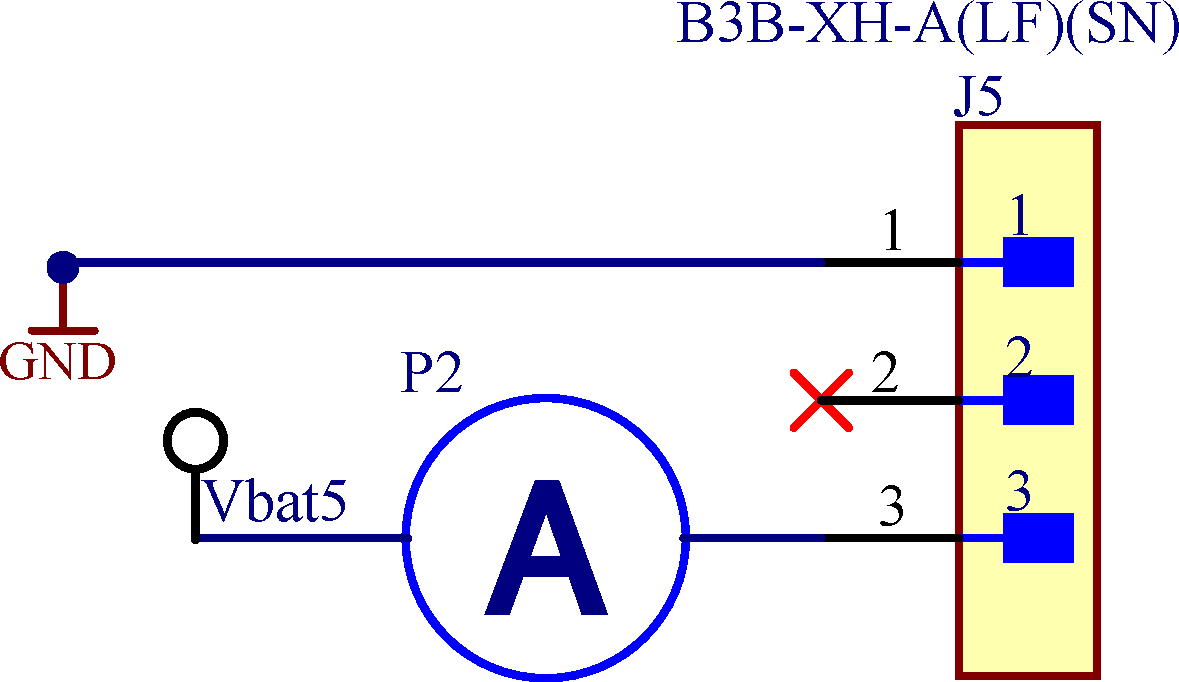
\includegraphics[width=.32\linewidth]{../figures/mesures/schema-courant}
	\caption{Schéma de mesure, courant}
	\label{fig:schema-courant}
	\source{Auteur}
\end{figure}

\subsubsection{Mesures}

\begin{table}[!h]
	\centering
	\resizebox{.78\textwidth}{!}{%
		\begin{tabular}{|c|l|l|c|c|}
			\hline
			\multicolumn{1}{|l|}{Index} & Etat du système & Condition                      & Courant [mA] & Symbol      \\ \hline
			[1]                         & Eteint.         & Mode auto-enclenchement OFF.   & 0.02         & $I_{off}$   \\ \hline
			[2]                         & Veille.         & Est passé par l'état SHUTDOWN. & 4.4          & $I_{sleep}$ \\ \hline
			[3]                         & Veille brutale.\footnotemark & Pas passé par l'état SHUTDOWN. & 9.56         & $I_{ws}$    \\ \hline
			[4]                         & Initialisation. & -                              & 90           & $I_{init}$  \\ \hline
			[5]                         & Logging.        & -                              & 100          & $I_{log}$   \\ \hline
			[6]                         & Shutdown.       & -                              & 83           & $I_{sh}$    \\ \hline
			[7]                         & Communication.  & USB branché.                   & 0            & $I_{usb}$   \\ \hline
		\end{tabular}%
	}
	\caption{Mesure des consommations}
	\label{tab:mes-cons}
	\source{Auteur}
\end{table}

\footnotetext{Lorsque le système a été éteint de façon non-contrôlée (Batterie débranchée).}

Nous pouvons par les mesure de la table \ref{tab:mes-cons} déduire les éléments suivants : 

Où : 

Capacité de la batterie $C = 1600\;mAh$

\begin{tabular}{llll}
	$\bullet$ & Temps de logging &  (Table \ref{tab:mes-cons}-[5]) : & $T_l = \frac{C}{I_{log}} = 16h$. \\
	$\bullet$ & Temps épuisement batterie en veille & (Table \ref{tab:mes-cons}-[2]) : & $T_l = \frac{C}{I_{sleep}} = 364h = 15J$. \\
	$\bullet$ & Temps épuisement en veille brutale & (Table \ref{tab:mes-cons}-[3]) : & $T_l = \frac{C}{I_{ws}} = 167h = 7J$. \\
\end{tabular}

Par conséquent, les caractéristiques d'autonomie de la batterie sont suffisantes pour notre application. 

\paragraph{Proposition de stratégies d'économie d'énergie}
Afin de diminuer la consommation lors du mode veille il existe différentes possibilités :

\noindent\textbf{Débraser la LED de la carte BNO0555 d'adafruit}

\begin{figure}[!h]
	\centering
	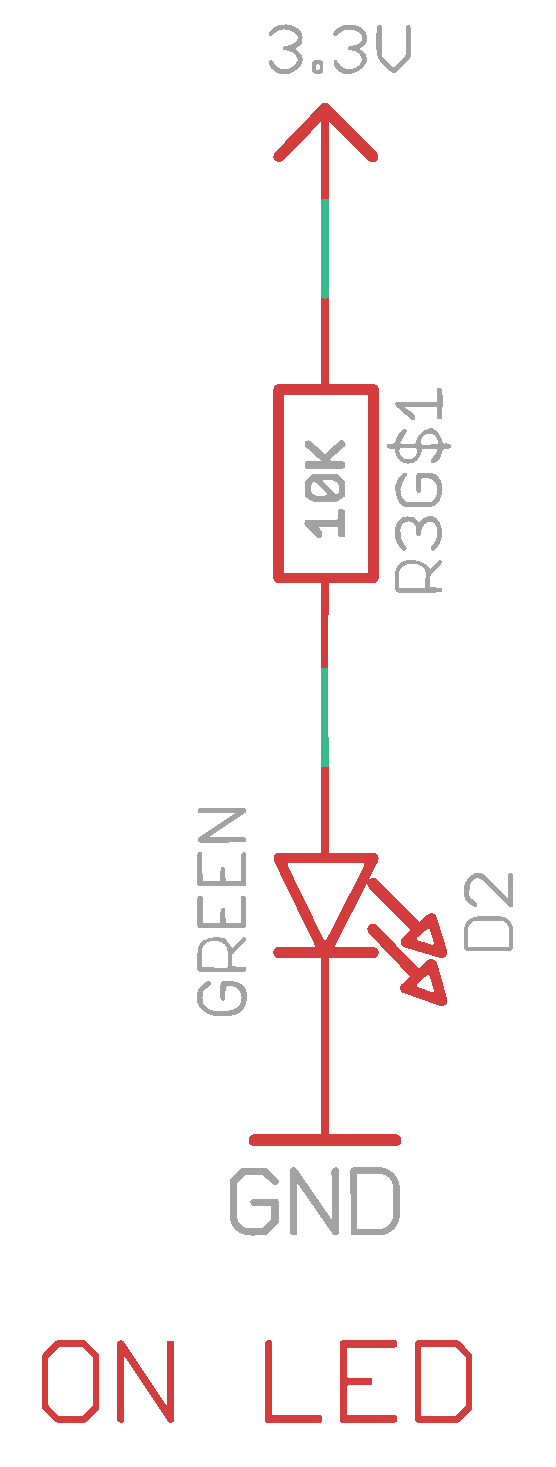
\includegraphics[width=0.16\linewidth]{../figures/mesures/led-imu}
	\caption{LED de vie de la carte d'adafruit (2.2V).}
	\label{fig:led-imu}
	\source{Schéma de la \href{https://cdn-learn.adafruit.com/assets/assets/000/092/544/original/sensors_BNO055_STEMMA_sch.png?1593120280}{carte BNO055 d'adafruit }}
\end{figure}

Comme le montre la figure \ref{fig:led-imu}, une LED reste constamment allumée lors de la mise sous tension de la carte de l'\gls{imu}. Elle présente une différence de potentiel de $2.2V$ à ses bornes, entraînant une consommation constante de \underline{$0.11mA$}. Bien que cette consommation soit faible, elle est inutile. Dans le cadre de ce prototype, la LED n'a pas été débrasée, mais un adhésif a été collé dessus afin de limiter la pollution lumineuse sur la LED d'état qui passe par un guide-lumière.

\noindent\textbf{Permettre de changer de mode plus facilement} Permettre à l'utilisateur de facilement basculer entre le mode "auto-enclenchement" et "enclenchement manuel" permettrait d'éviter des consommations inutiles.



\subsection{Bus de communications}
Avec le code implémenté dans le microcontrôleur, les différents périphériques fonctionnent correctement et la communication avec les différents bus est opérationnelle. C'est pourquoi, dans cette section, l'objectif principal est de mesurer la qualité et l'intégrité des signaux plutôt que d'analyser les différents protocoles.

\subsubsection{Communication I2C} \label{ssec:Comm-I2C}
La communication I2C s'effectue entre la centrale inertielle BNO055 et le microcontrôleur. Par ce bus, les configurations du registre de l'\gls{imu} ainsi que les données inertielles mesurées, en fonction de ces configurations, sont transmises. Comme nous avons pu le voir précédemment, cette communication est effective et les données sont cohérentes. Dans ce contexte, nous examinerons si l'intervalle entre les mesures est respecté, la durée de ces mesures, ainsi que la qualité des signaux I2C.


\paragraph{Méthode de mesure}
La boîte noire a été configurée pour transmettre et enregistrer des données inertielles à intervalles de 2 secondes. De plus, les mesures ont été prises pendant la transmission des données inertielles, et non lors de la configuration. Enfin, les trames ont été décodées automatiquement par l'oscilloscope grâce à sa fonction "Protocol".

\paragraph{Schéma de mesure} Le schéma de mesure est présenté sur la figure \ref{fig:schema-mesure-i2c}.


\begin{figure}[H]
	\centering
	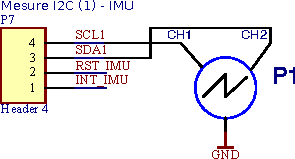
\includegraphics[width=0.4\linewidth]{../figures/mesures/I2C/Schema-mesure-i2c}
	\caption{Schéma de mesure, mesures I2C.}
	\label{fig:schema-mesure-i2c}
	\source{Auteur}
\end{figure}

\paragraph{Mesures}
Comme le montre la figure \ref{fig:intervale-2s}, il y a un délai de \underline{$1.98$} secondes entre l'envoi de deux sets de données de la centrale inertielle.


\begin{figure}[H]
	\centering
	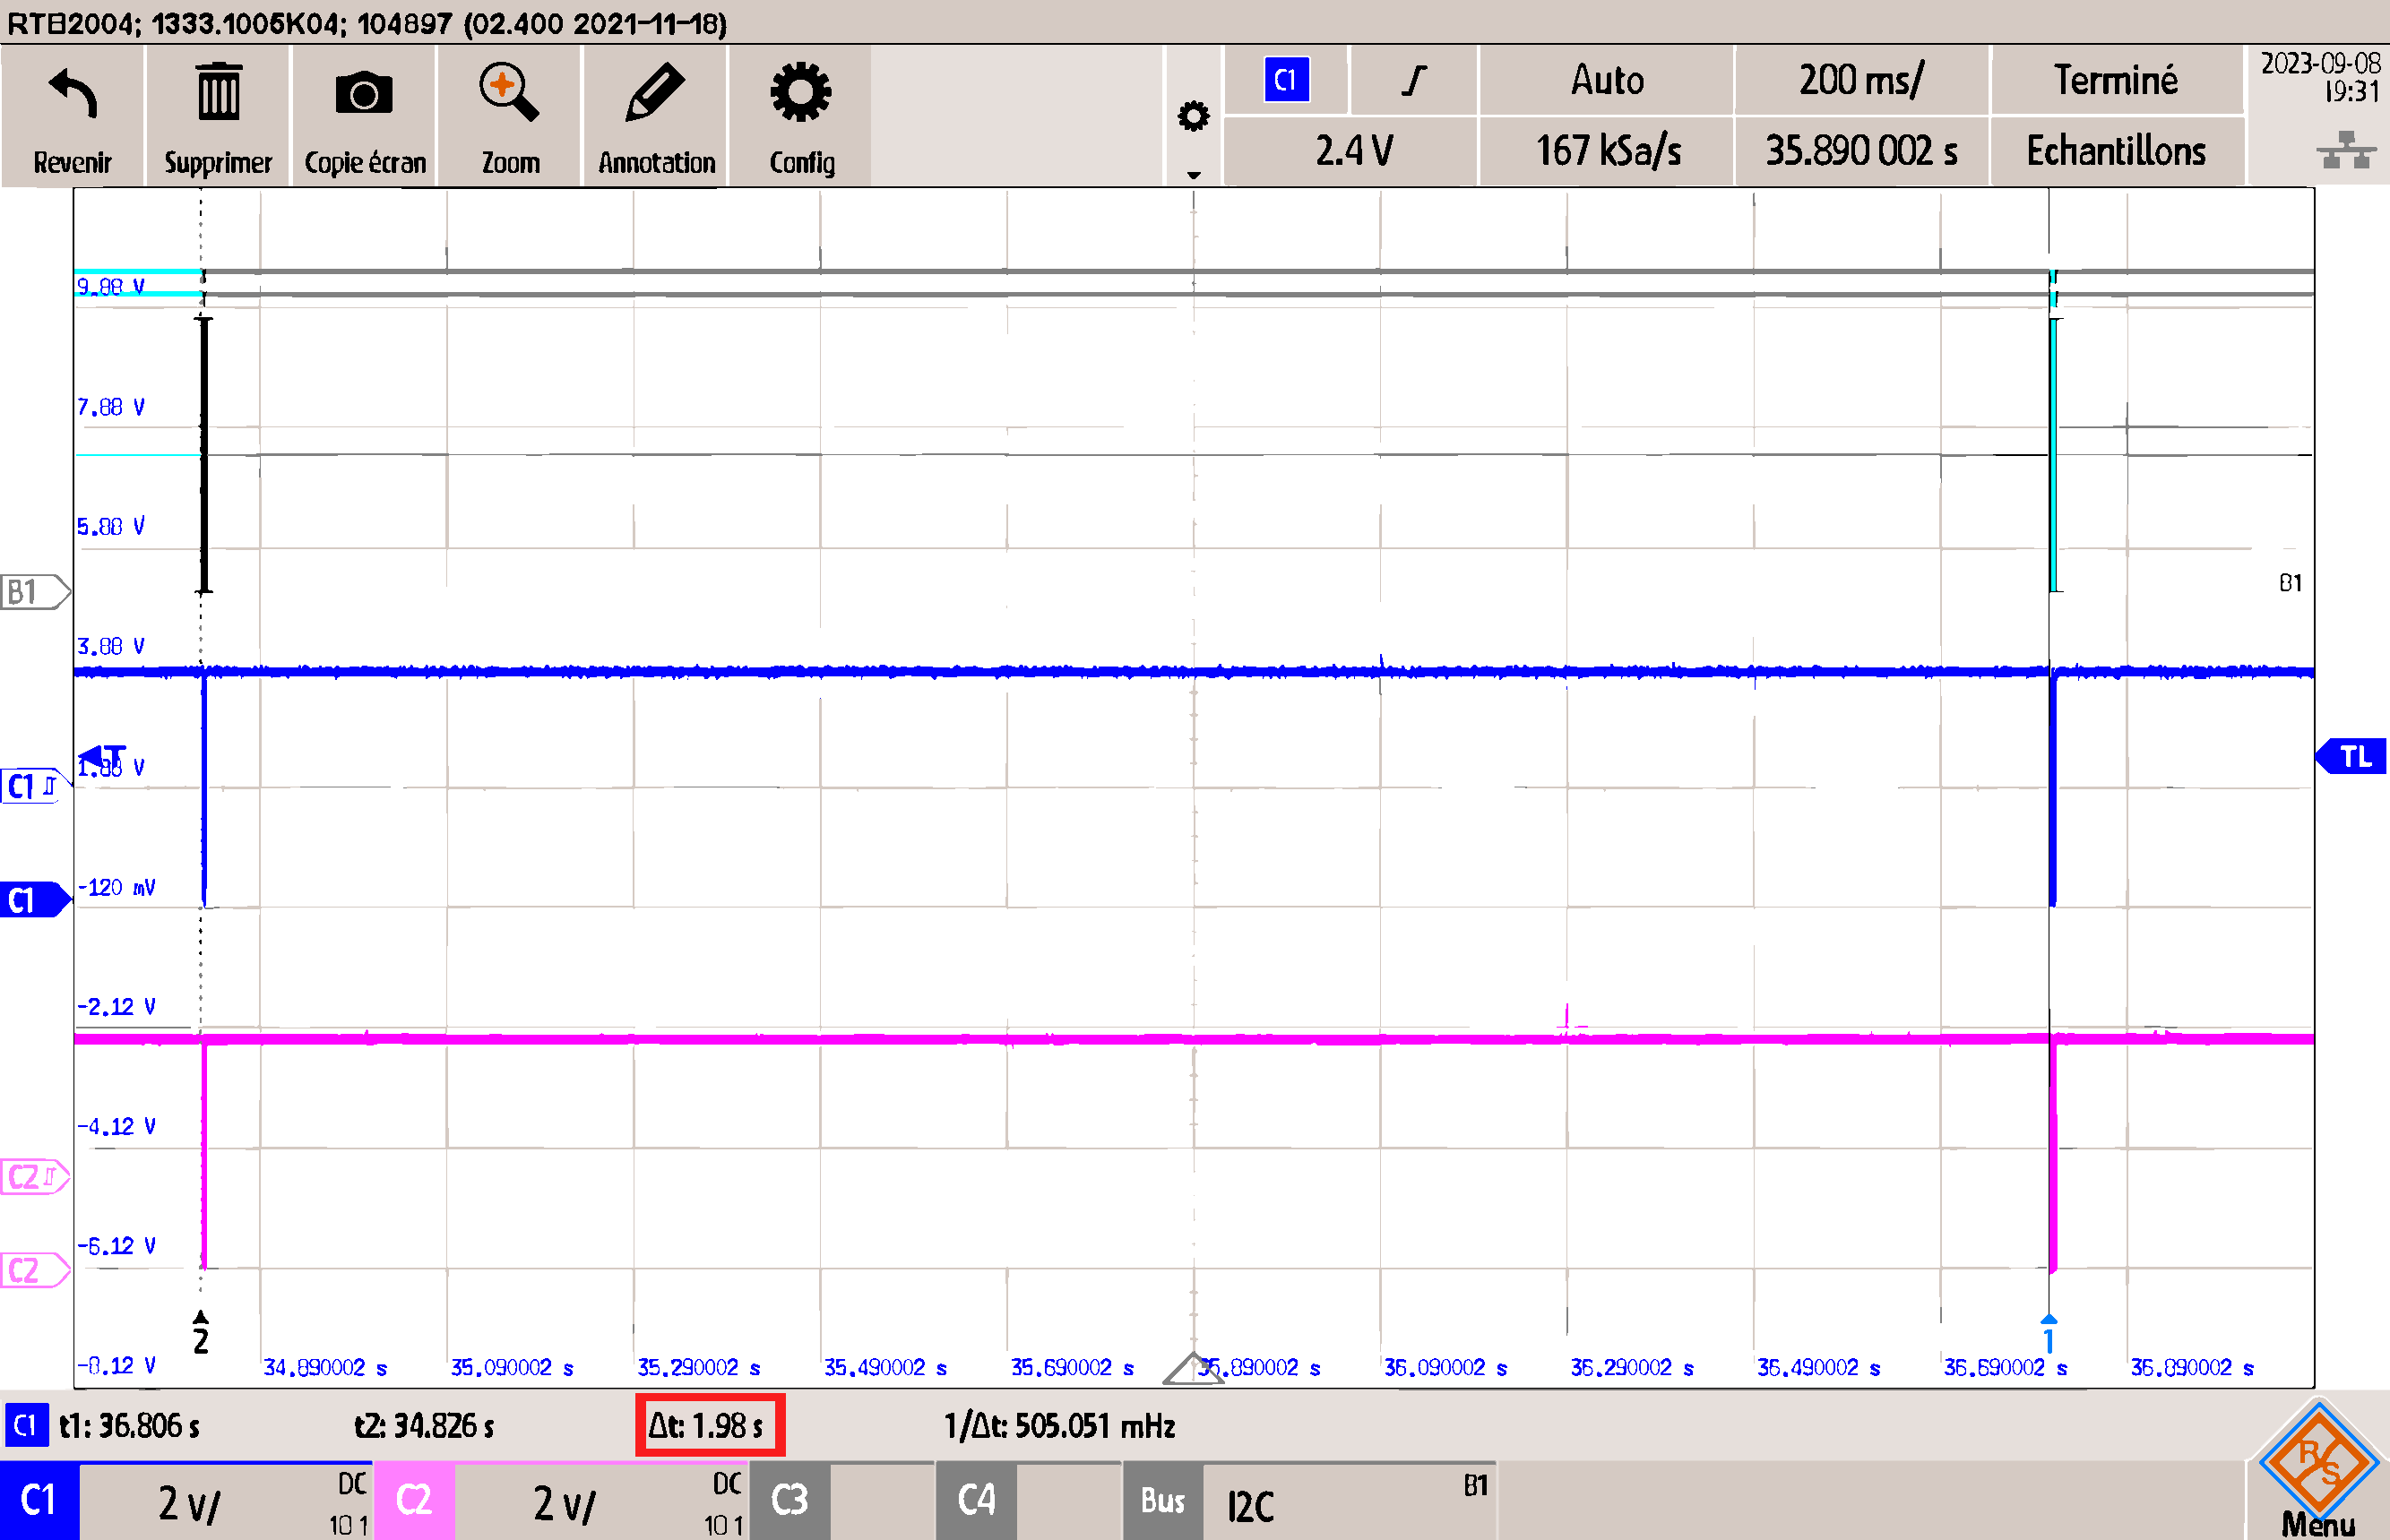
\includegraphics[width=.7\linewidth]{../figures/mesures/I2C/Intervale-2s}
	\caption{Intervale entre deux mesures, config. 2 secondes.}
	\label{fig:intervale-2s}
	\source{Auteur}
\end{figure}

Malgré la légère différence sur la figure \ref{fig:intervale-2s} de $20ms$, probablement due à une imprécision de mesure, nous pouvons conclure que l'intervalle entre les mesures respecte bien la configuration établie, même après modifications de celle-ci.

Sur la figure \ref{fig:duree-comm}, nous observons la durée d'une trame de mesures qui englobe toutes les données mentionnées dans la section \ref{sssec:IMU-data}. La durée de transmission d'un set de mesure est de \underline{$2.274ms$}. Compte tenu que le bus est configuré en mode "fast" à $400 kbit/s$, cela suggère qu'environ $\sim910$ bits ont été transmis, ce qui explique la densité des données rendant la figure peu lisible.

\begin{figure}[H]
	\centering
	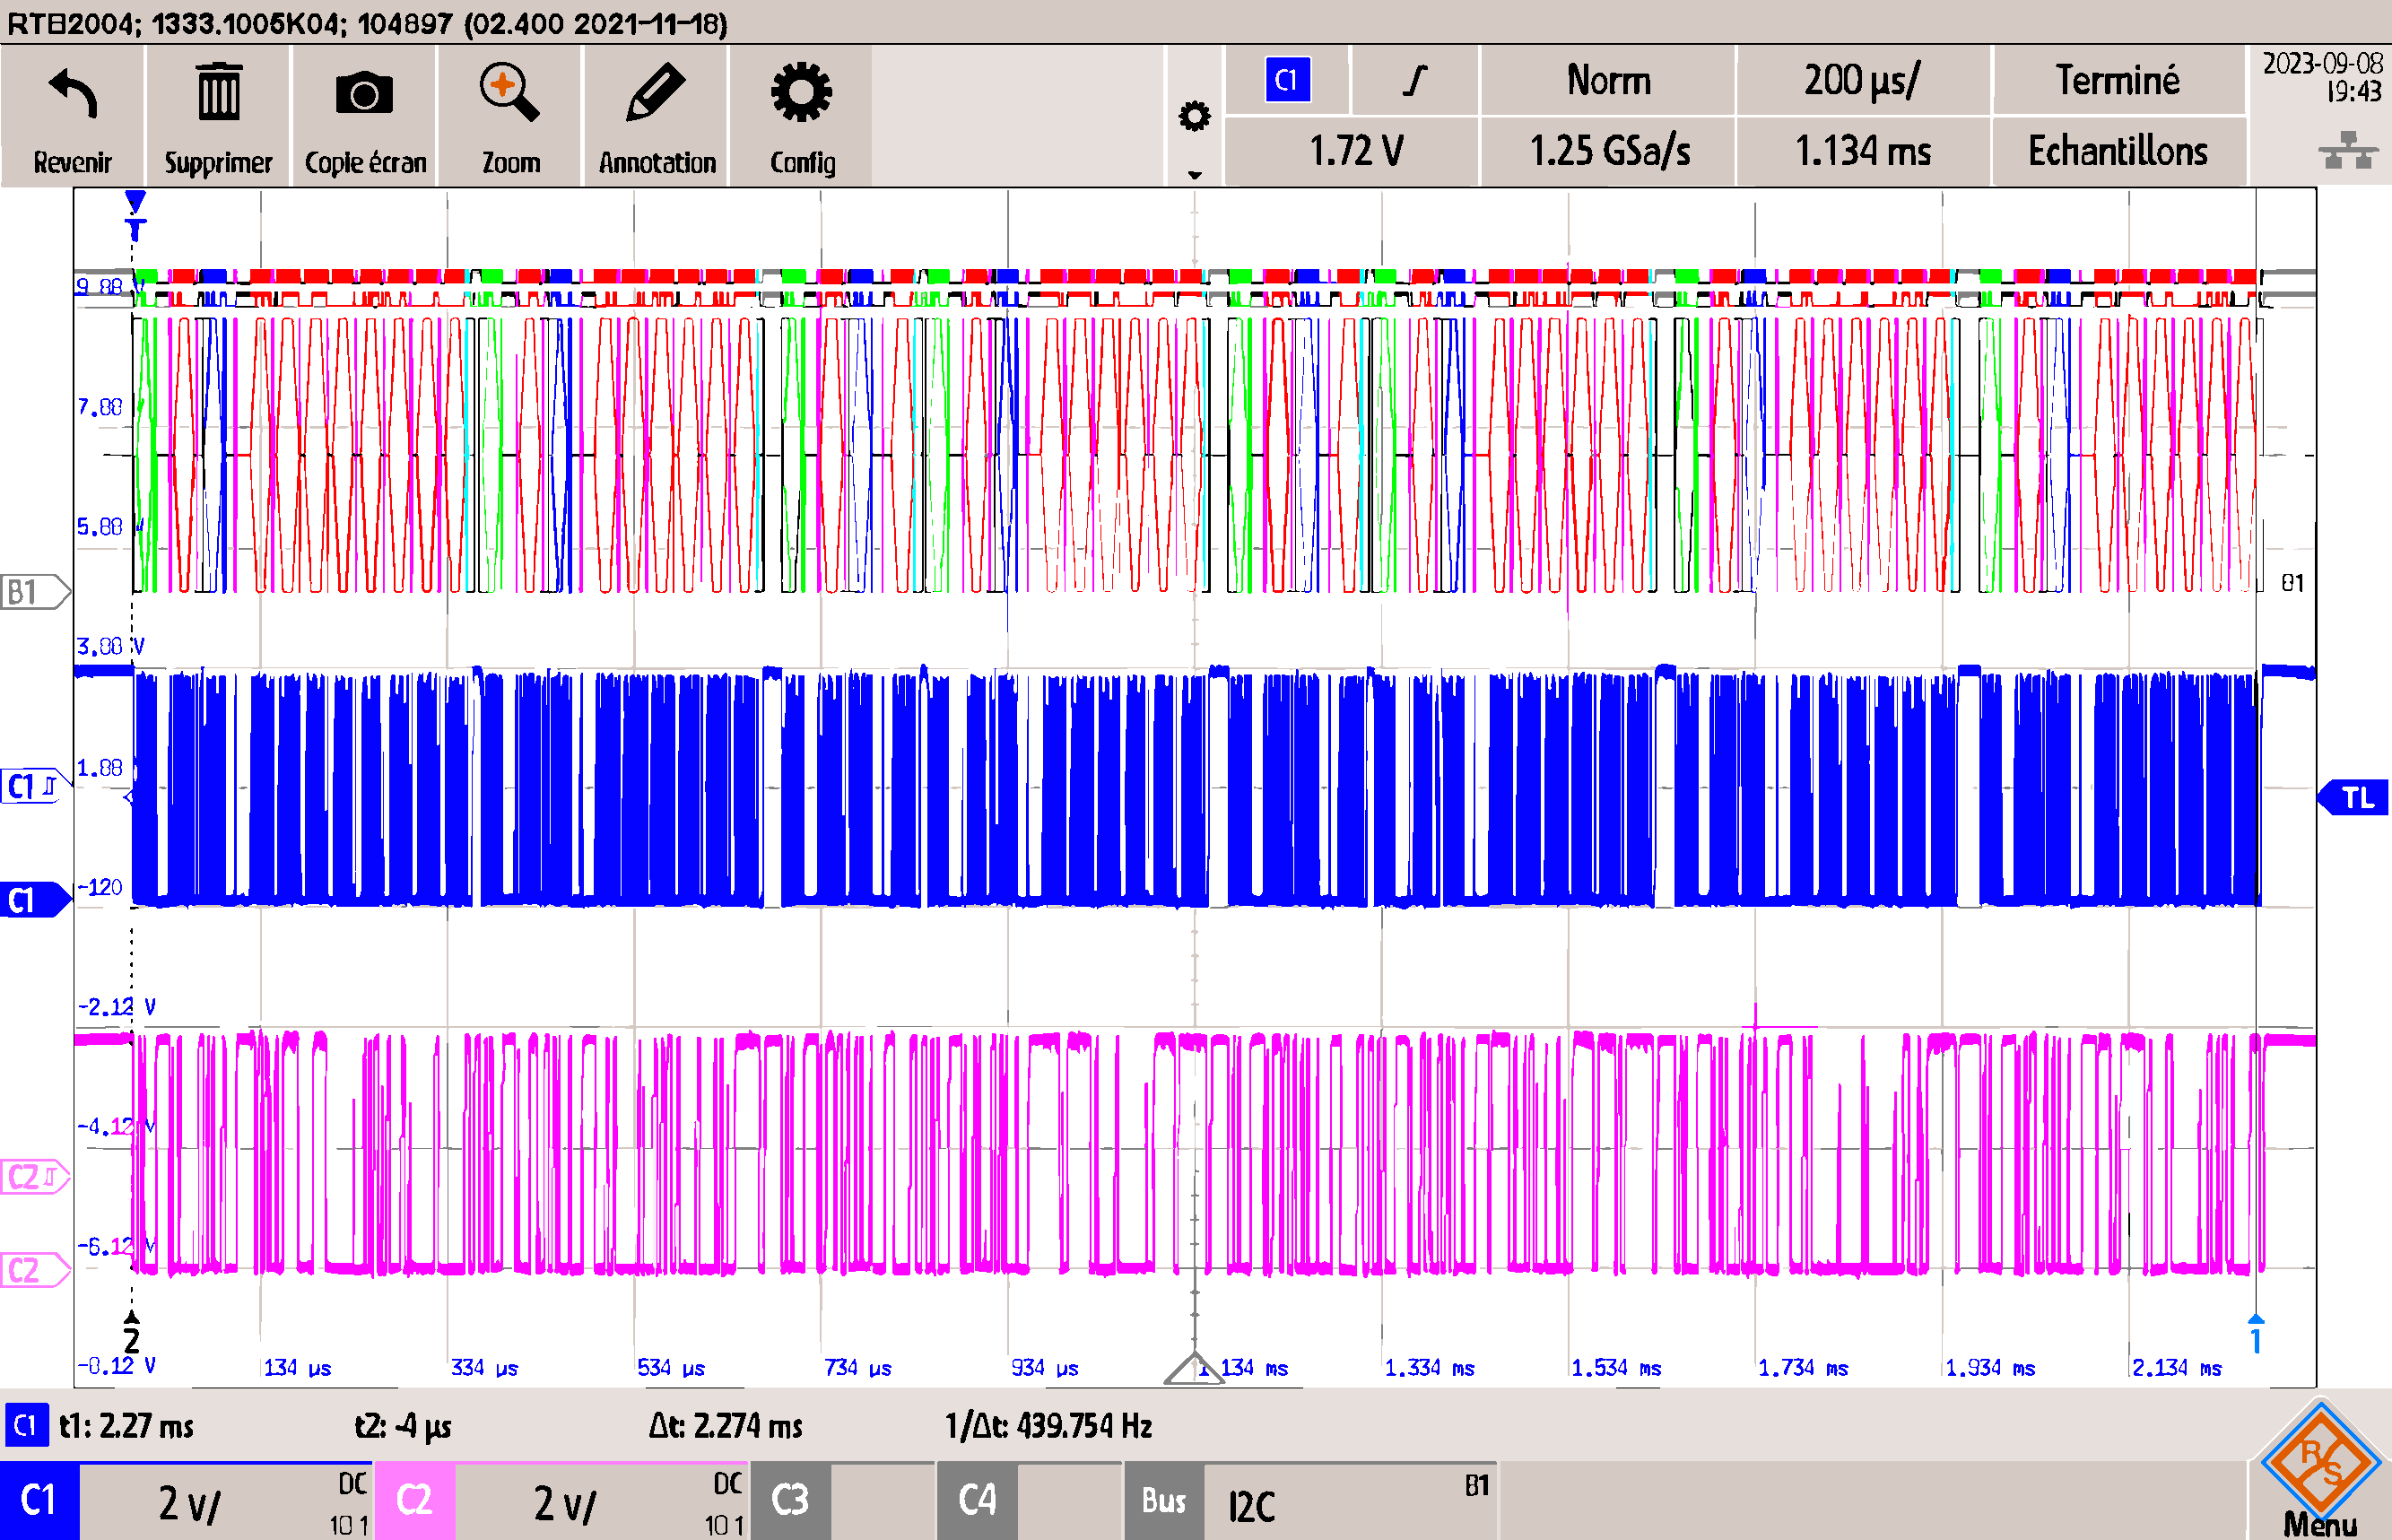
\includegraphics[width=.7\linewidth]{../figures/mesures/I2C/duree-comm}
	\caption{Durée d'une mesure.}
	\label{fig:duree-comm}
	\source{Auteur}
\end{figure}

Sur la figure \ref{fig:tramme-mesure}, nous observons le début d'une communication avec l'\gls{imu}. Le premier byte (\textbf{0x28}) correspond à l'adresse du BNO055. Ensuite, le registre \textbf{0x28} est adressé : il s'agit du registre contenant les données \textbf{LSB} de l'accélération linéaire. Les flancs des bits transmis semblent suffisamment nettes et peu parasités pour une bonne communication.

\begin{figure}[H]
	\centering
	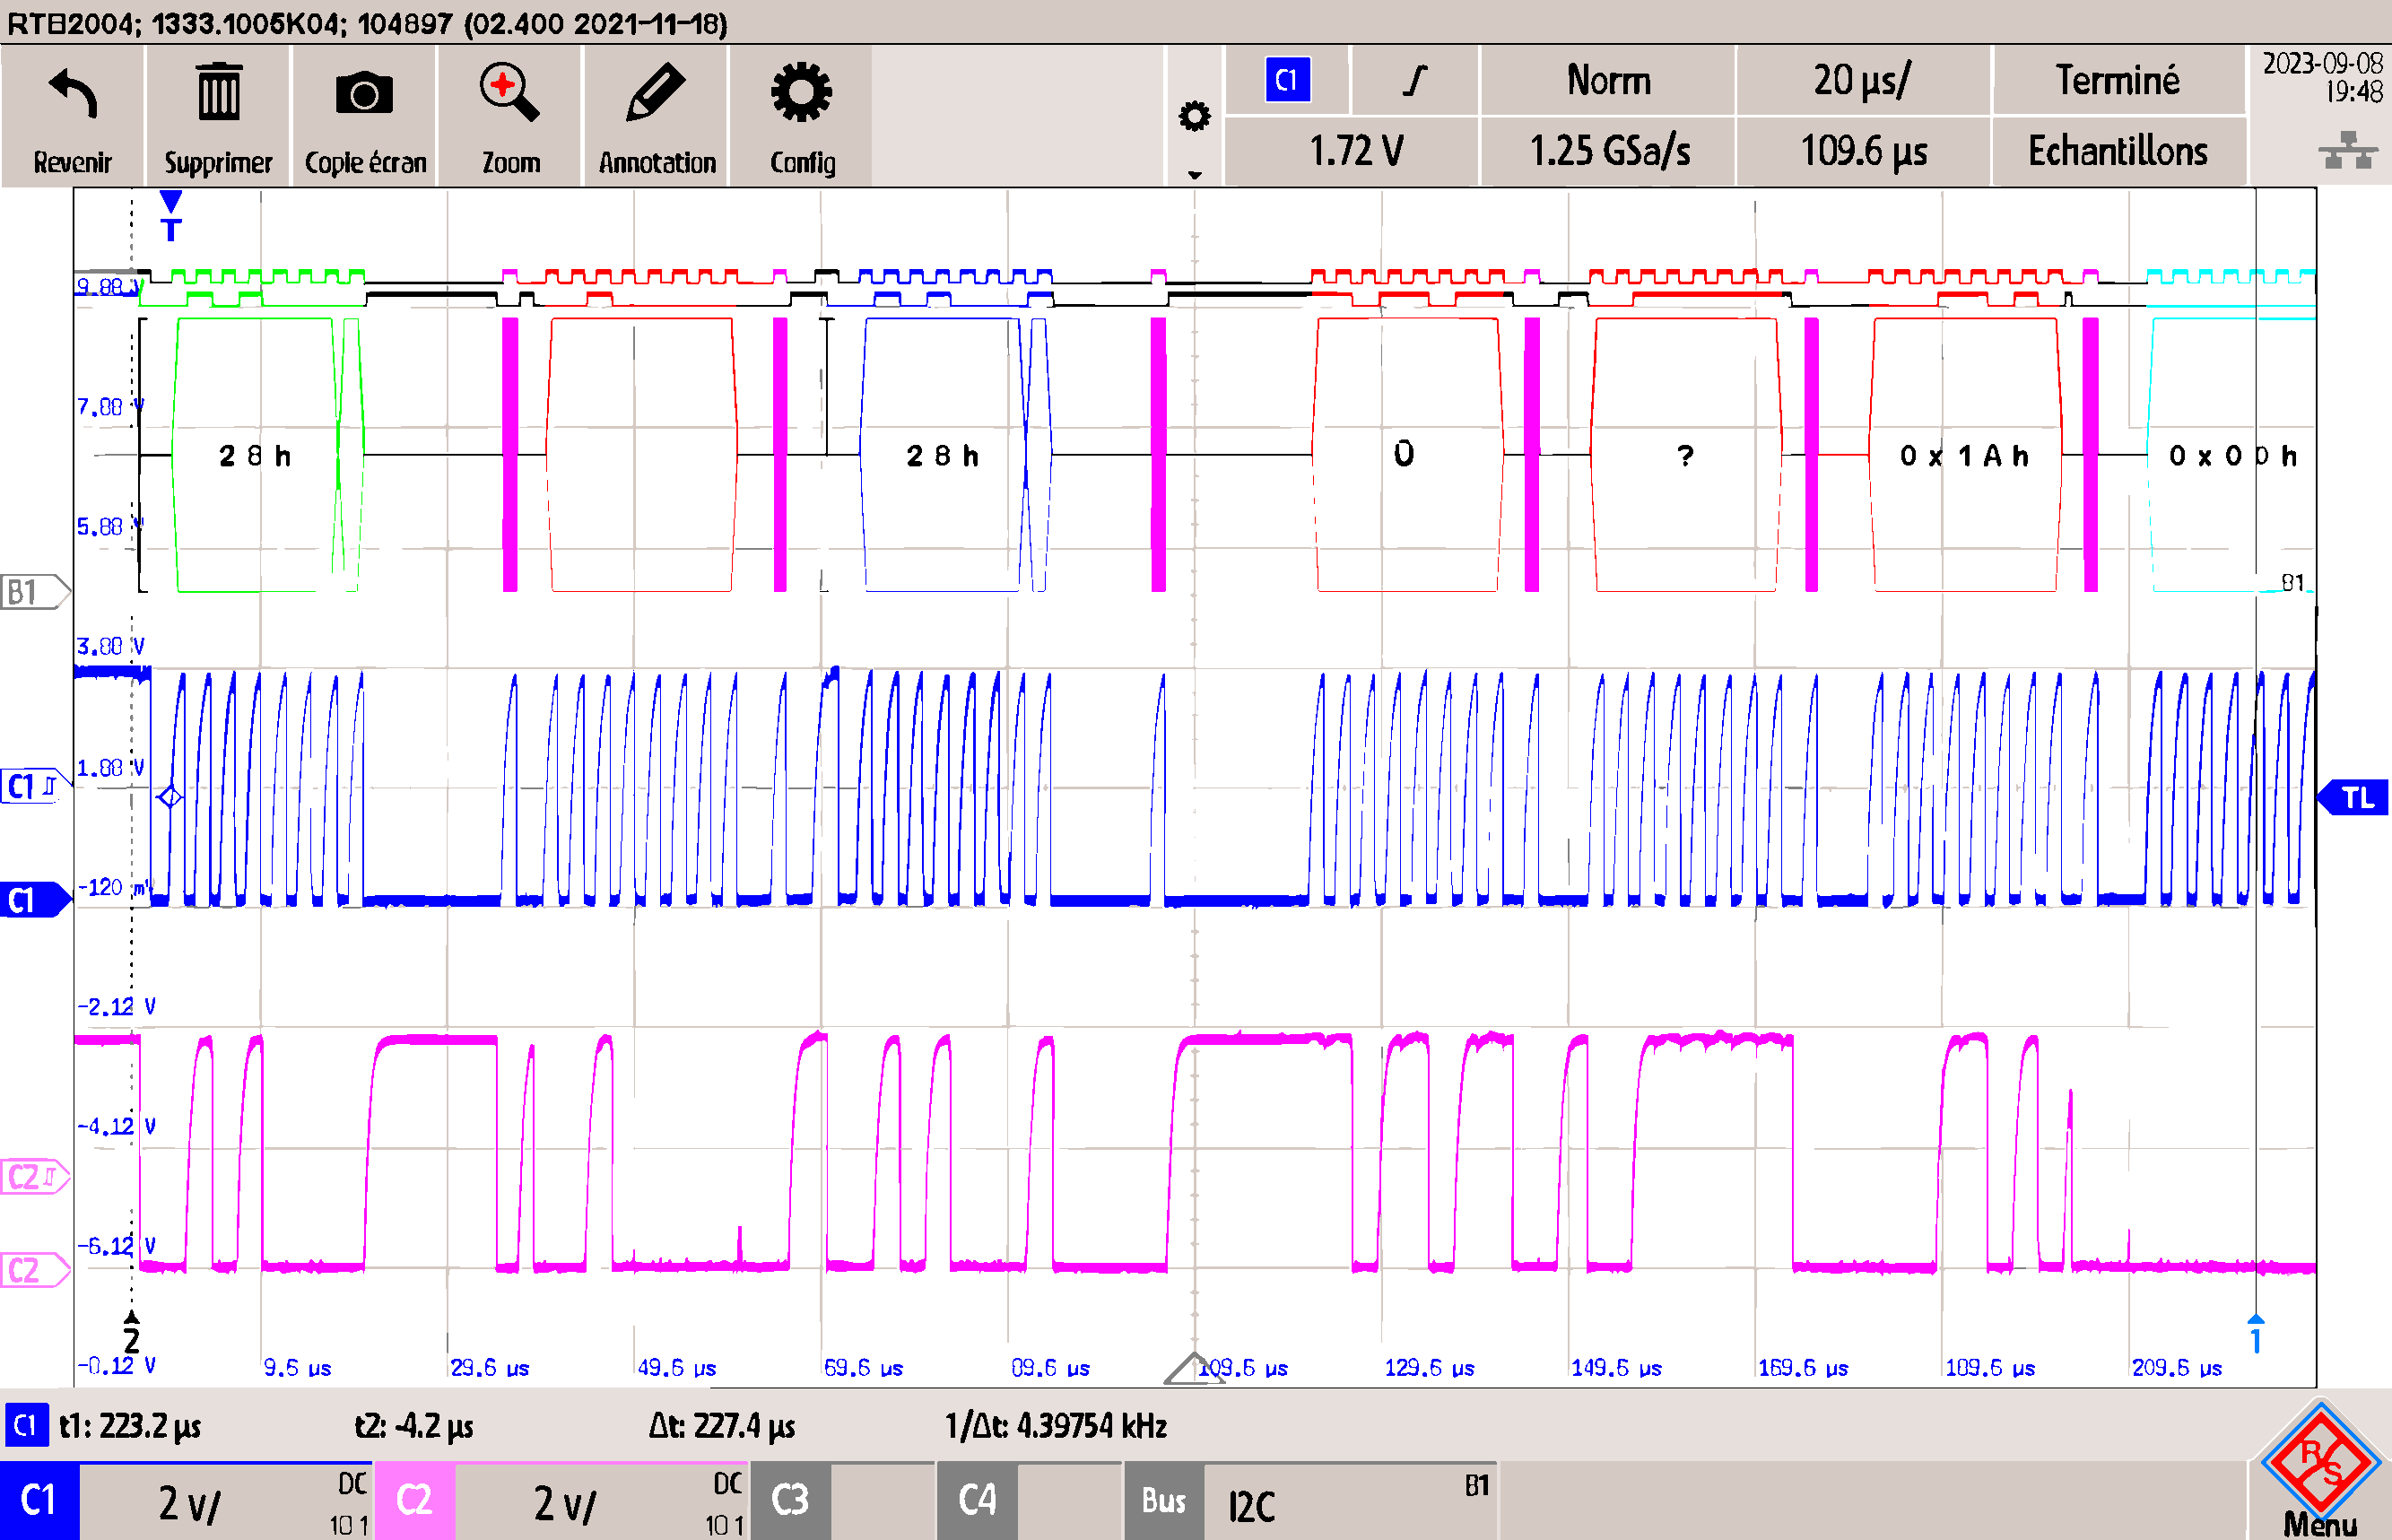
\includegraphics[width=.7\linewidth]{../figures/mesures/I2C/Tramme-mesure}
	\caption{Début de tramme d'une mesure.}
	\label{fig:tramme-mesure}
	\source{Auteur}
\end{figure}

\clearpage

\subsubsection{Communication UART GNSS} \label{ssec:Comm-UART}
Dans cette section, nous analyserons les différentes caractéristiques de la communication UART entre le microcontrôleur et le module \gls{gnss}.

\paragraph{Méthode de mesure} Pour réaliser ces mesures, le système a été activé et le \gls{gnss} a été configuré par défaut à une fréquence de \textbf{1Hz}.

\paragraph{Schéma de mesure} Le schéma de mesure est présenté sur la figure \ref{fig:scheam-mesure-uart-gnss}, nous nous intéressants ici, qu'au message envoyés par le GNSS dans sa configuration par défaut. 
\begin{figure}[h]
	\centering
	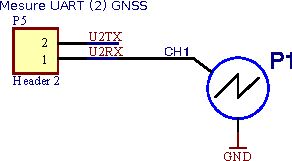
\includegraphics[width=0.4\linewidth]{../figures/mesures/UART/scheam-mesure-uart-gnss}
	\caption{Schéma de mesure \gls{gnss}.}
	\label{fig:scheam-mesure-uart-gnss}
	\source{Auteur}
\end{figure}



\paragraph{Mesures}
Sur la figure \ref{fig:interval-gnss}, nous observons l'intervalle entre les messages GNSS. Effectivement, cet intervalle est de \underline{$1s$}, offrant ainsi suffisamment de temps au \gls{mcu} pour traiter ces données, que ce soit pour les afficher sur un terminal ou les enregistrer sur la carte SD.

\begin{figure}[H]
	\centering
	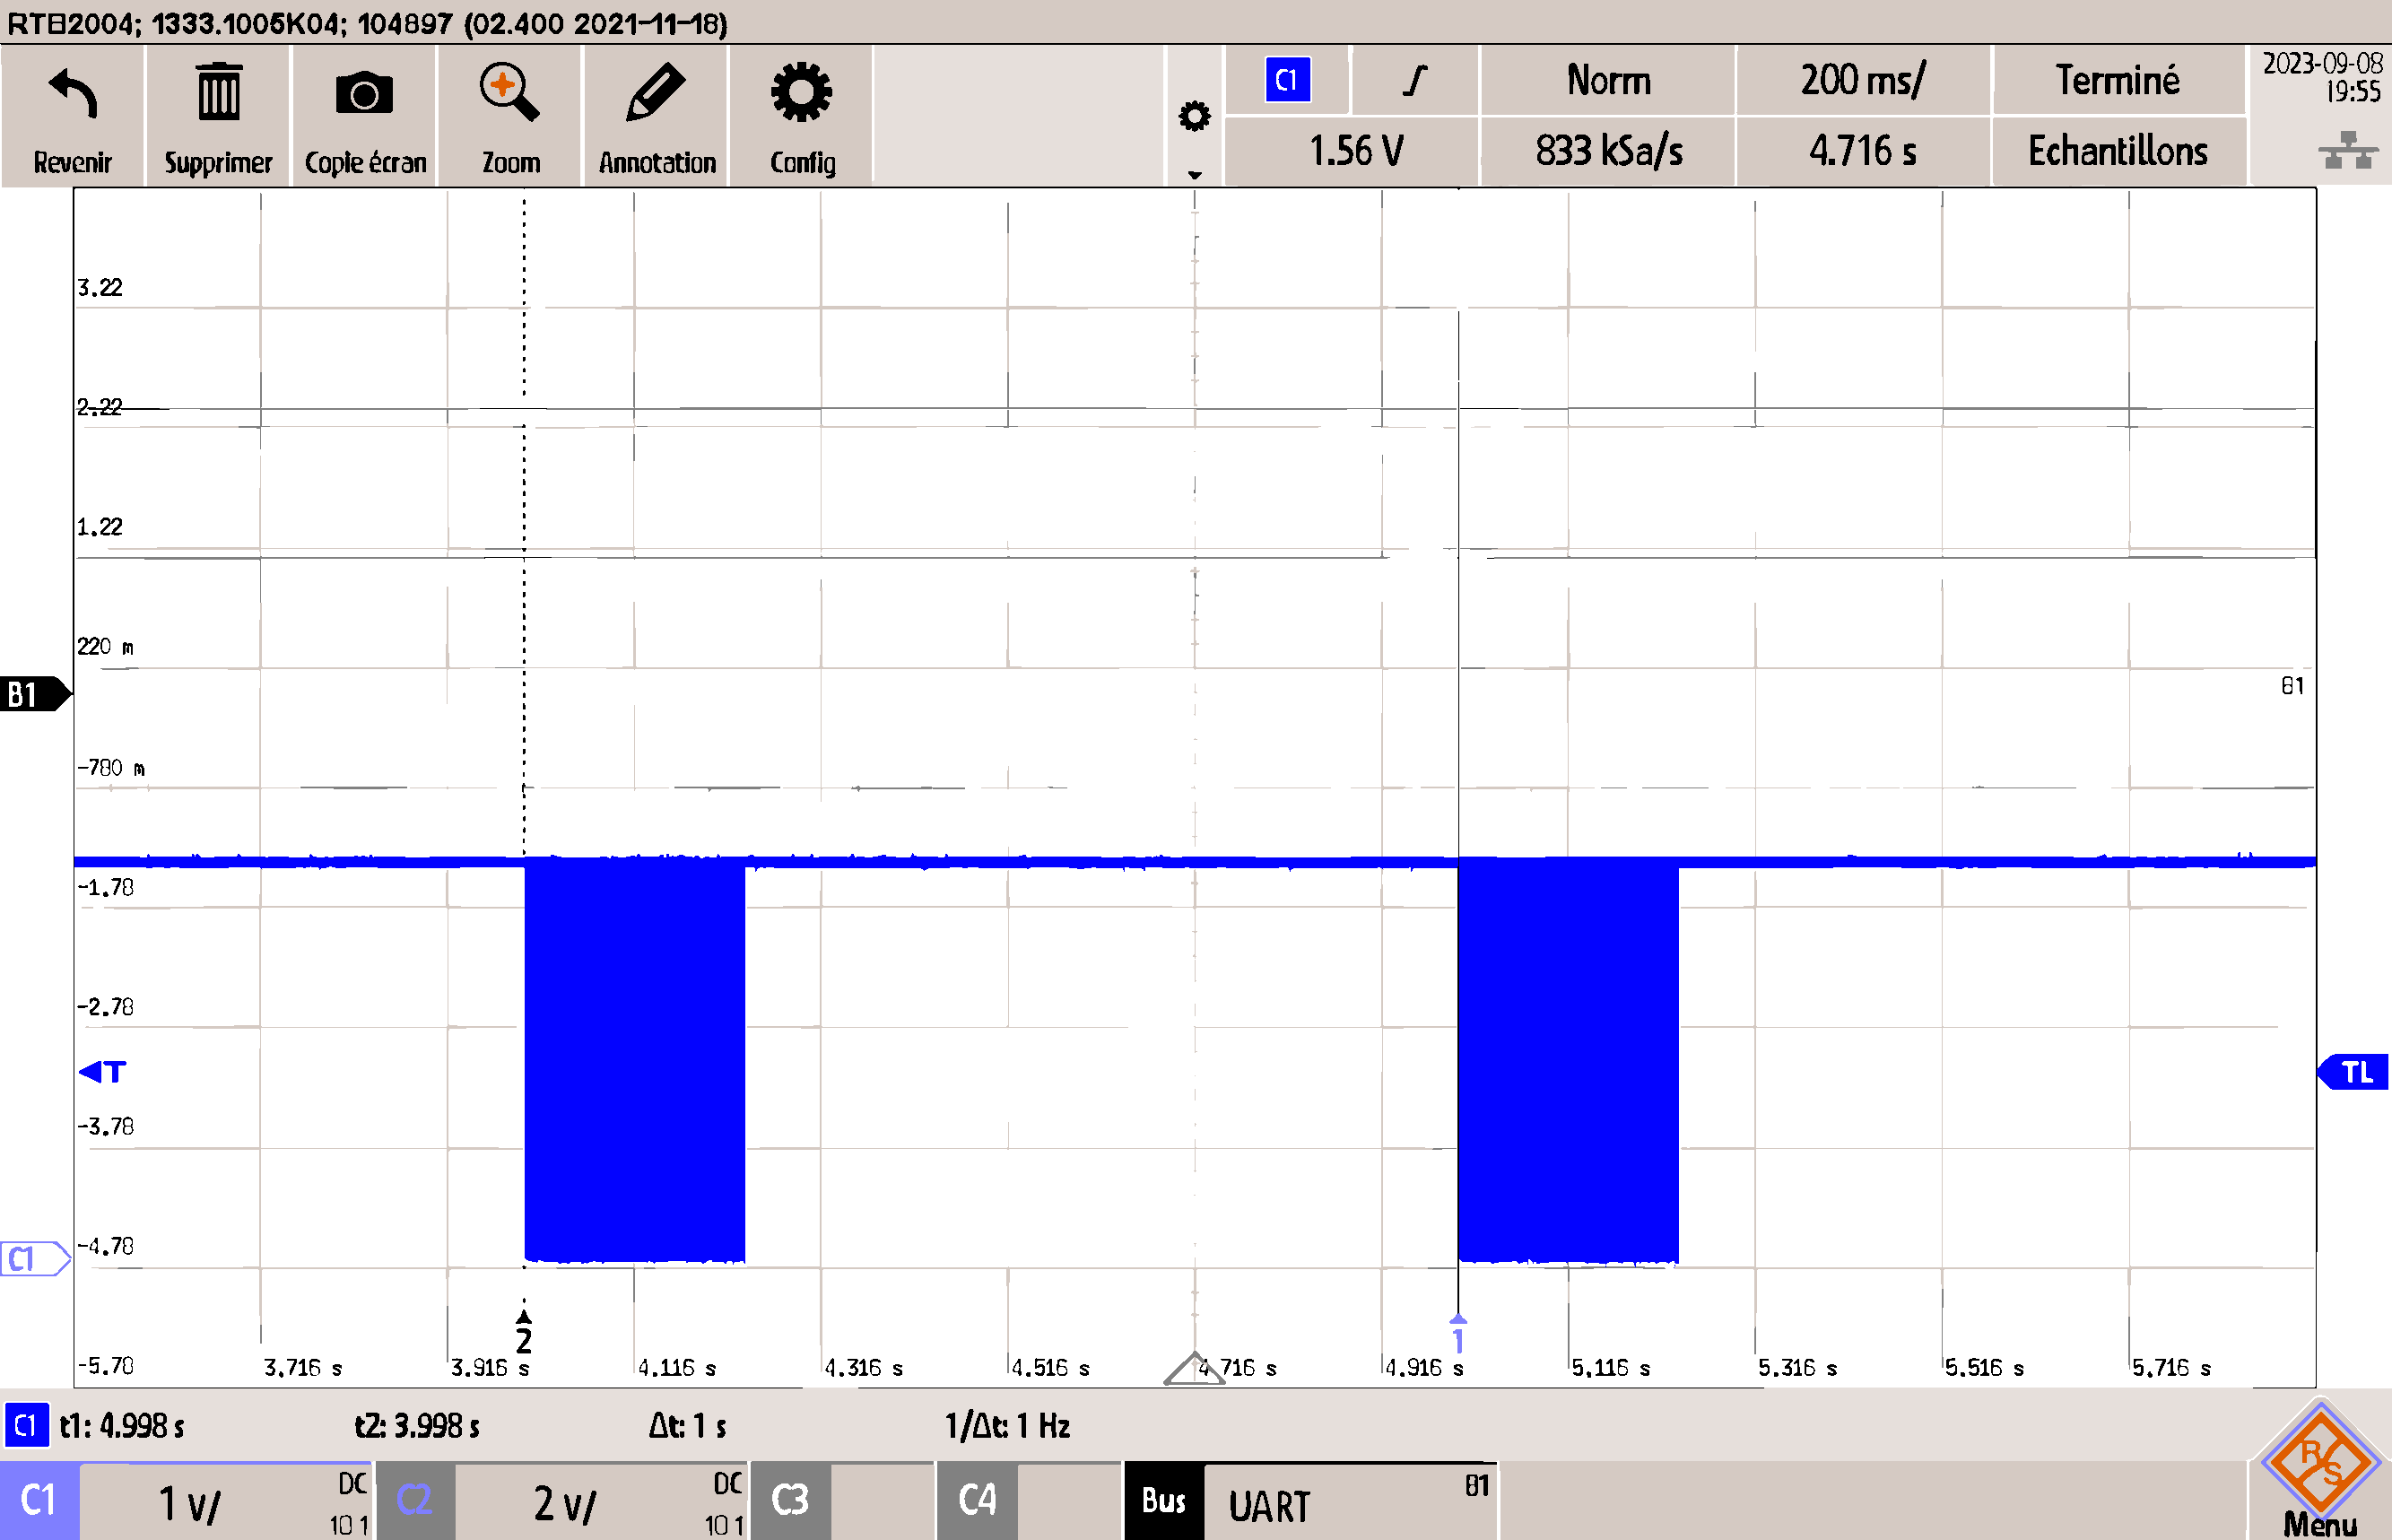
\includegraphics[width=0.7\linewidth]{../figures/mesures/UART/interval-gnss}
	\caption{Intervale entre les données NMEA.}
	\label{fig:interval-gnss}
	\source{Auteur}
\end{figure}

Sur la figure \ref{fig:duree-comm-gnss}, nous constatons que la durée d'envoi des messages \textbf{NMEA} est de \underline{$234.4 ms$}. Sachant que l'intervalle entre les transmissions est de \underline{$1s$}, cela laisse une fenêtre de $756ms$ au \gls{mcu} pour traiter ces données. Cette période est largement suffisante pour la transmission des données via le second UART (opérant au même baud rate) ou vers la carte SD, dont la fréquence est nettement supérieure ($10MHz$). Si nous considérons la durée des transmissions de l'\gls{imu}, qui est de \underline{$2.274ms$}, nous estimons avec une marge qu'environ $\sim400ms$ des $756ms$ disponibles sont utilisés pour traiter les données. Ce temps de traitement pourrait être encore diminuée si la fréquence d'enregistrement du \gls{gnss} était baissée. Ainsi, nous pourrions envisager d'obtenir jusqu'à $\sim155$ mesures d'\gls{imu} dans l'intervalle donné.


\begin{figure}[H]
	\centering
	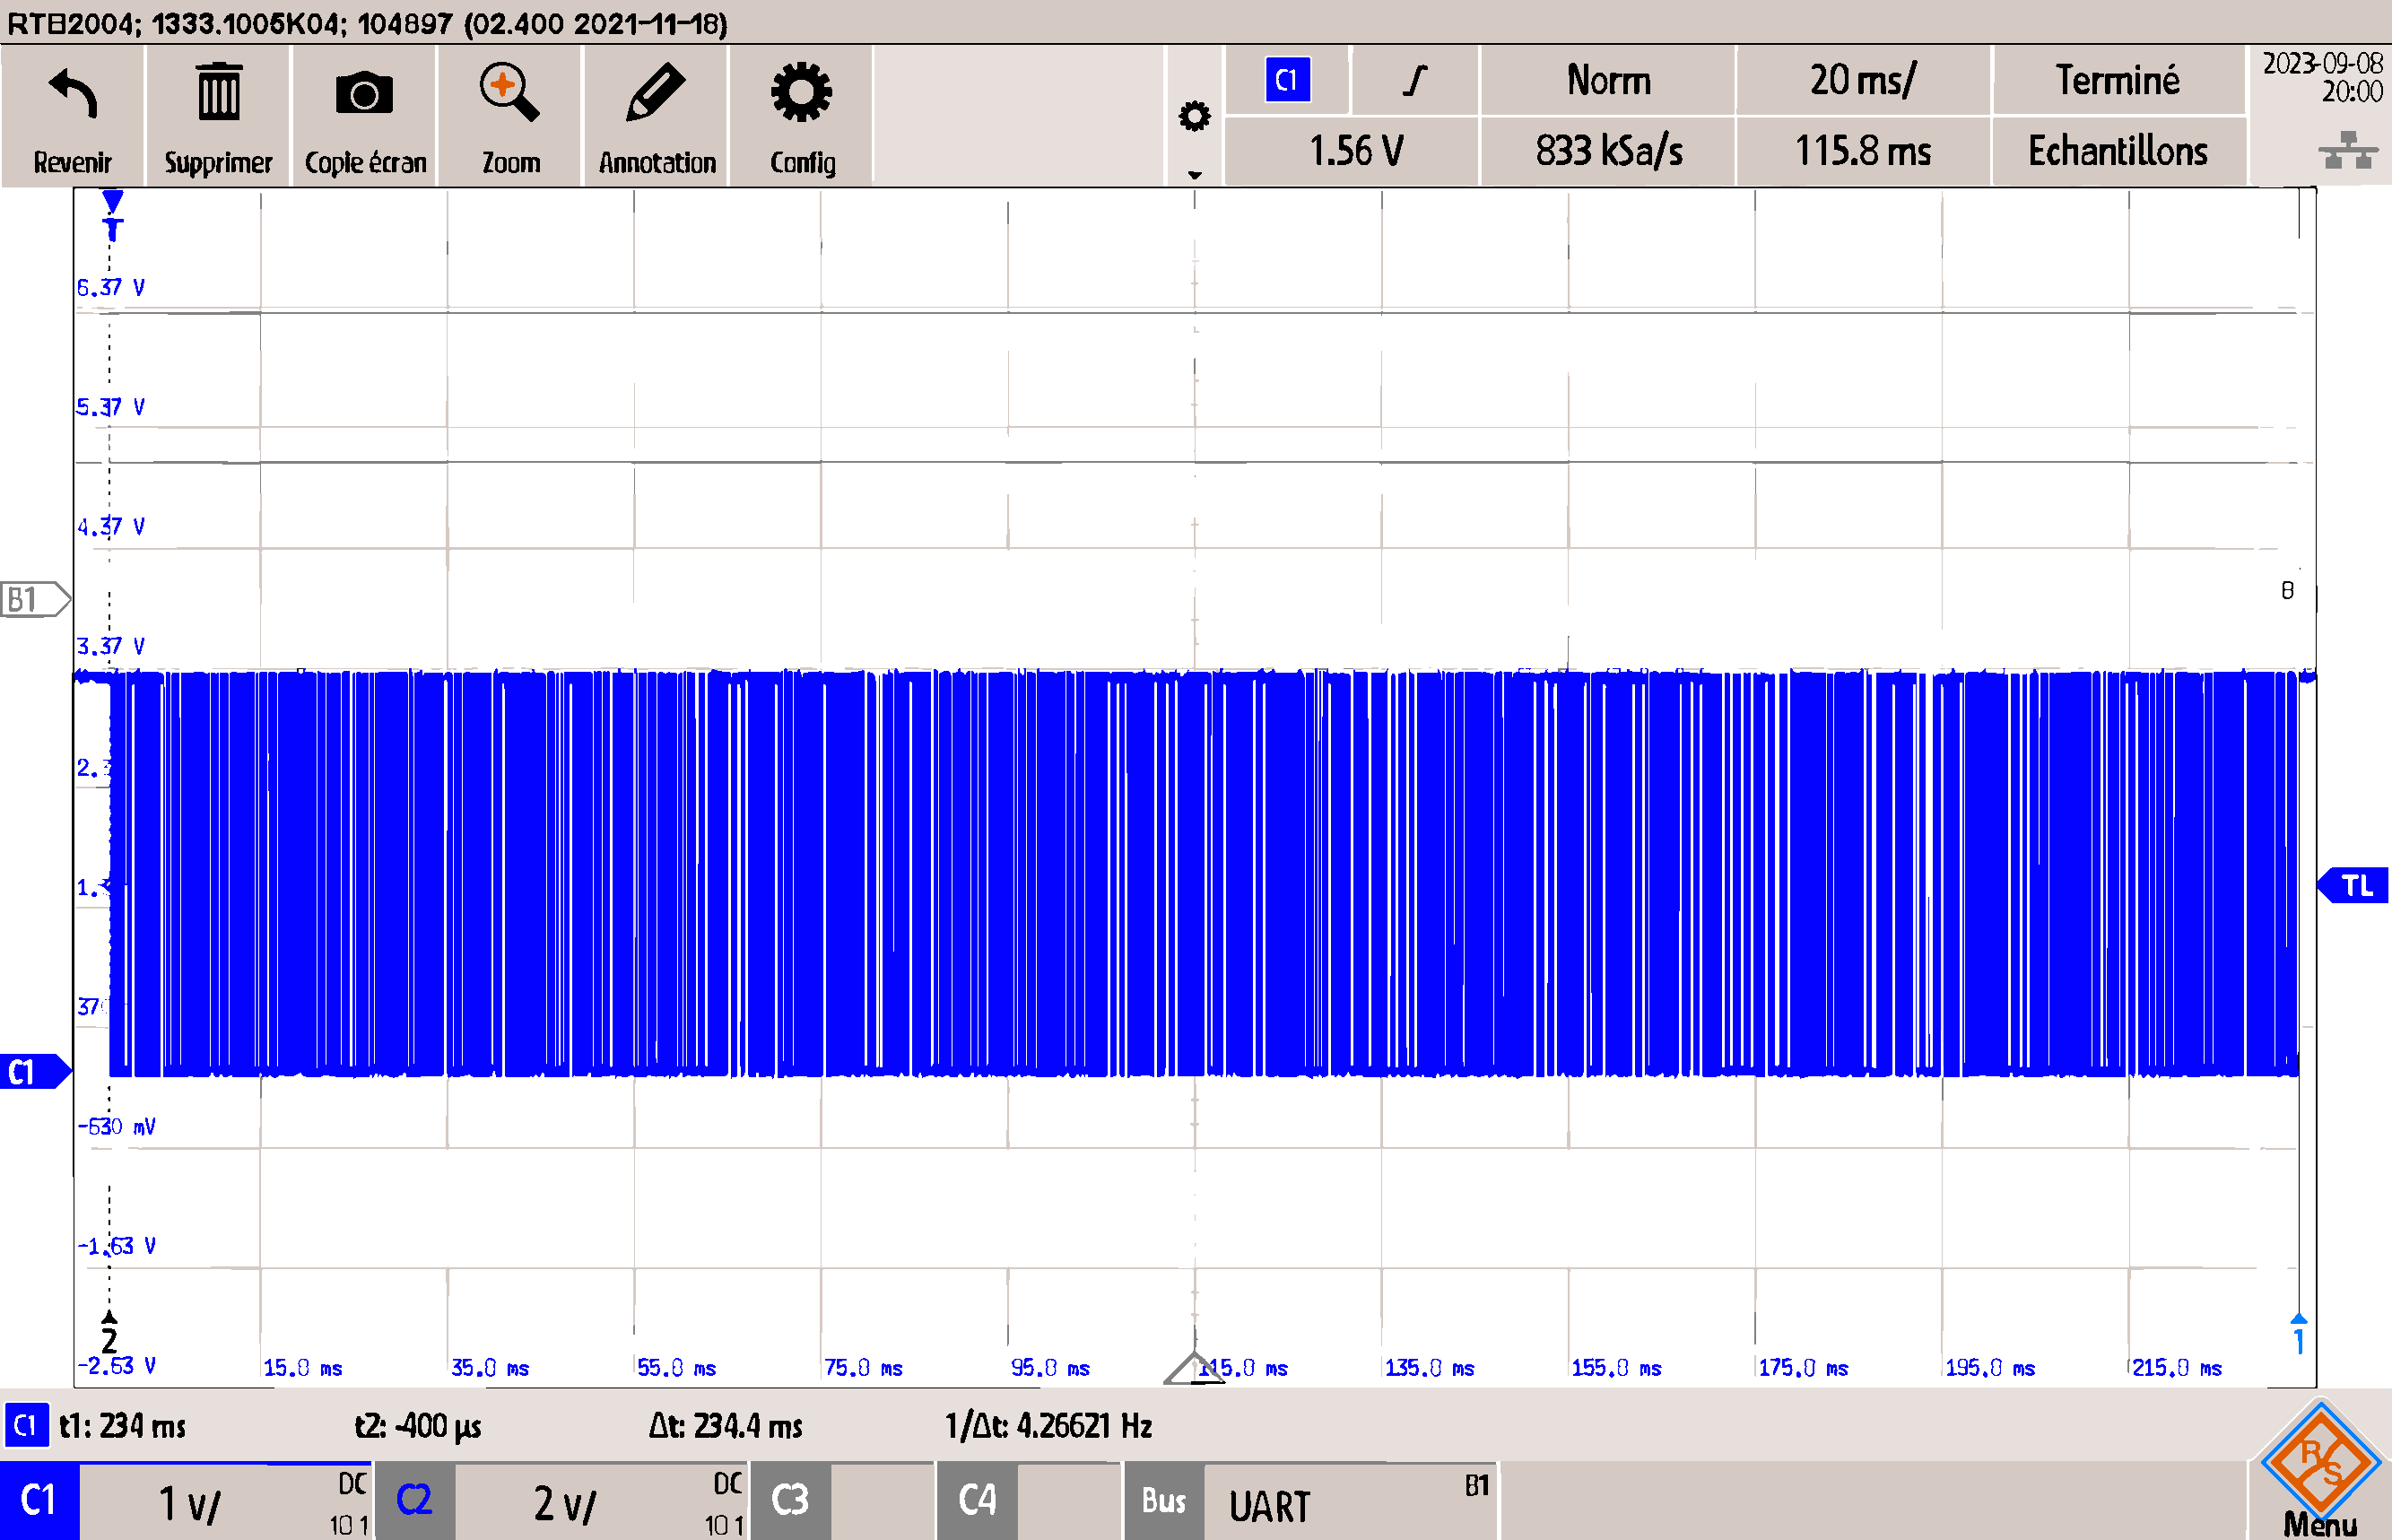
\includegraphics[width=0.7\linewidth]{../figures/mesures/UART/duree-comm-gnss}
	\caption{Durée d'une communication avec le GNSS.}
	\label{fig:duree-comm-gnss}
	\source{Auteur}
\end{figure}

La figure \ref{fig:message-nmea-rmc} illustre le décodage d'une trame \textbf{NMEA} correspondant à un message \textbf{RMC}. Les données de ce message sont similaires à celles présentées dans la section \ref{sssec:GNSS-data}. Les signaux présentent une bonne intégrité et sont correctement interprétés par le microcontrôleur. Ils sont ensuite retransmis à la carte SD et au second UART avec justesse.


\begin{figure}[H]
	\centering
	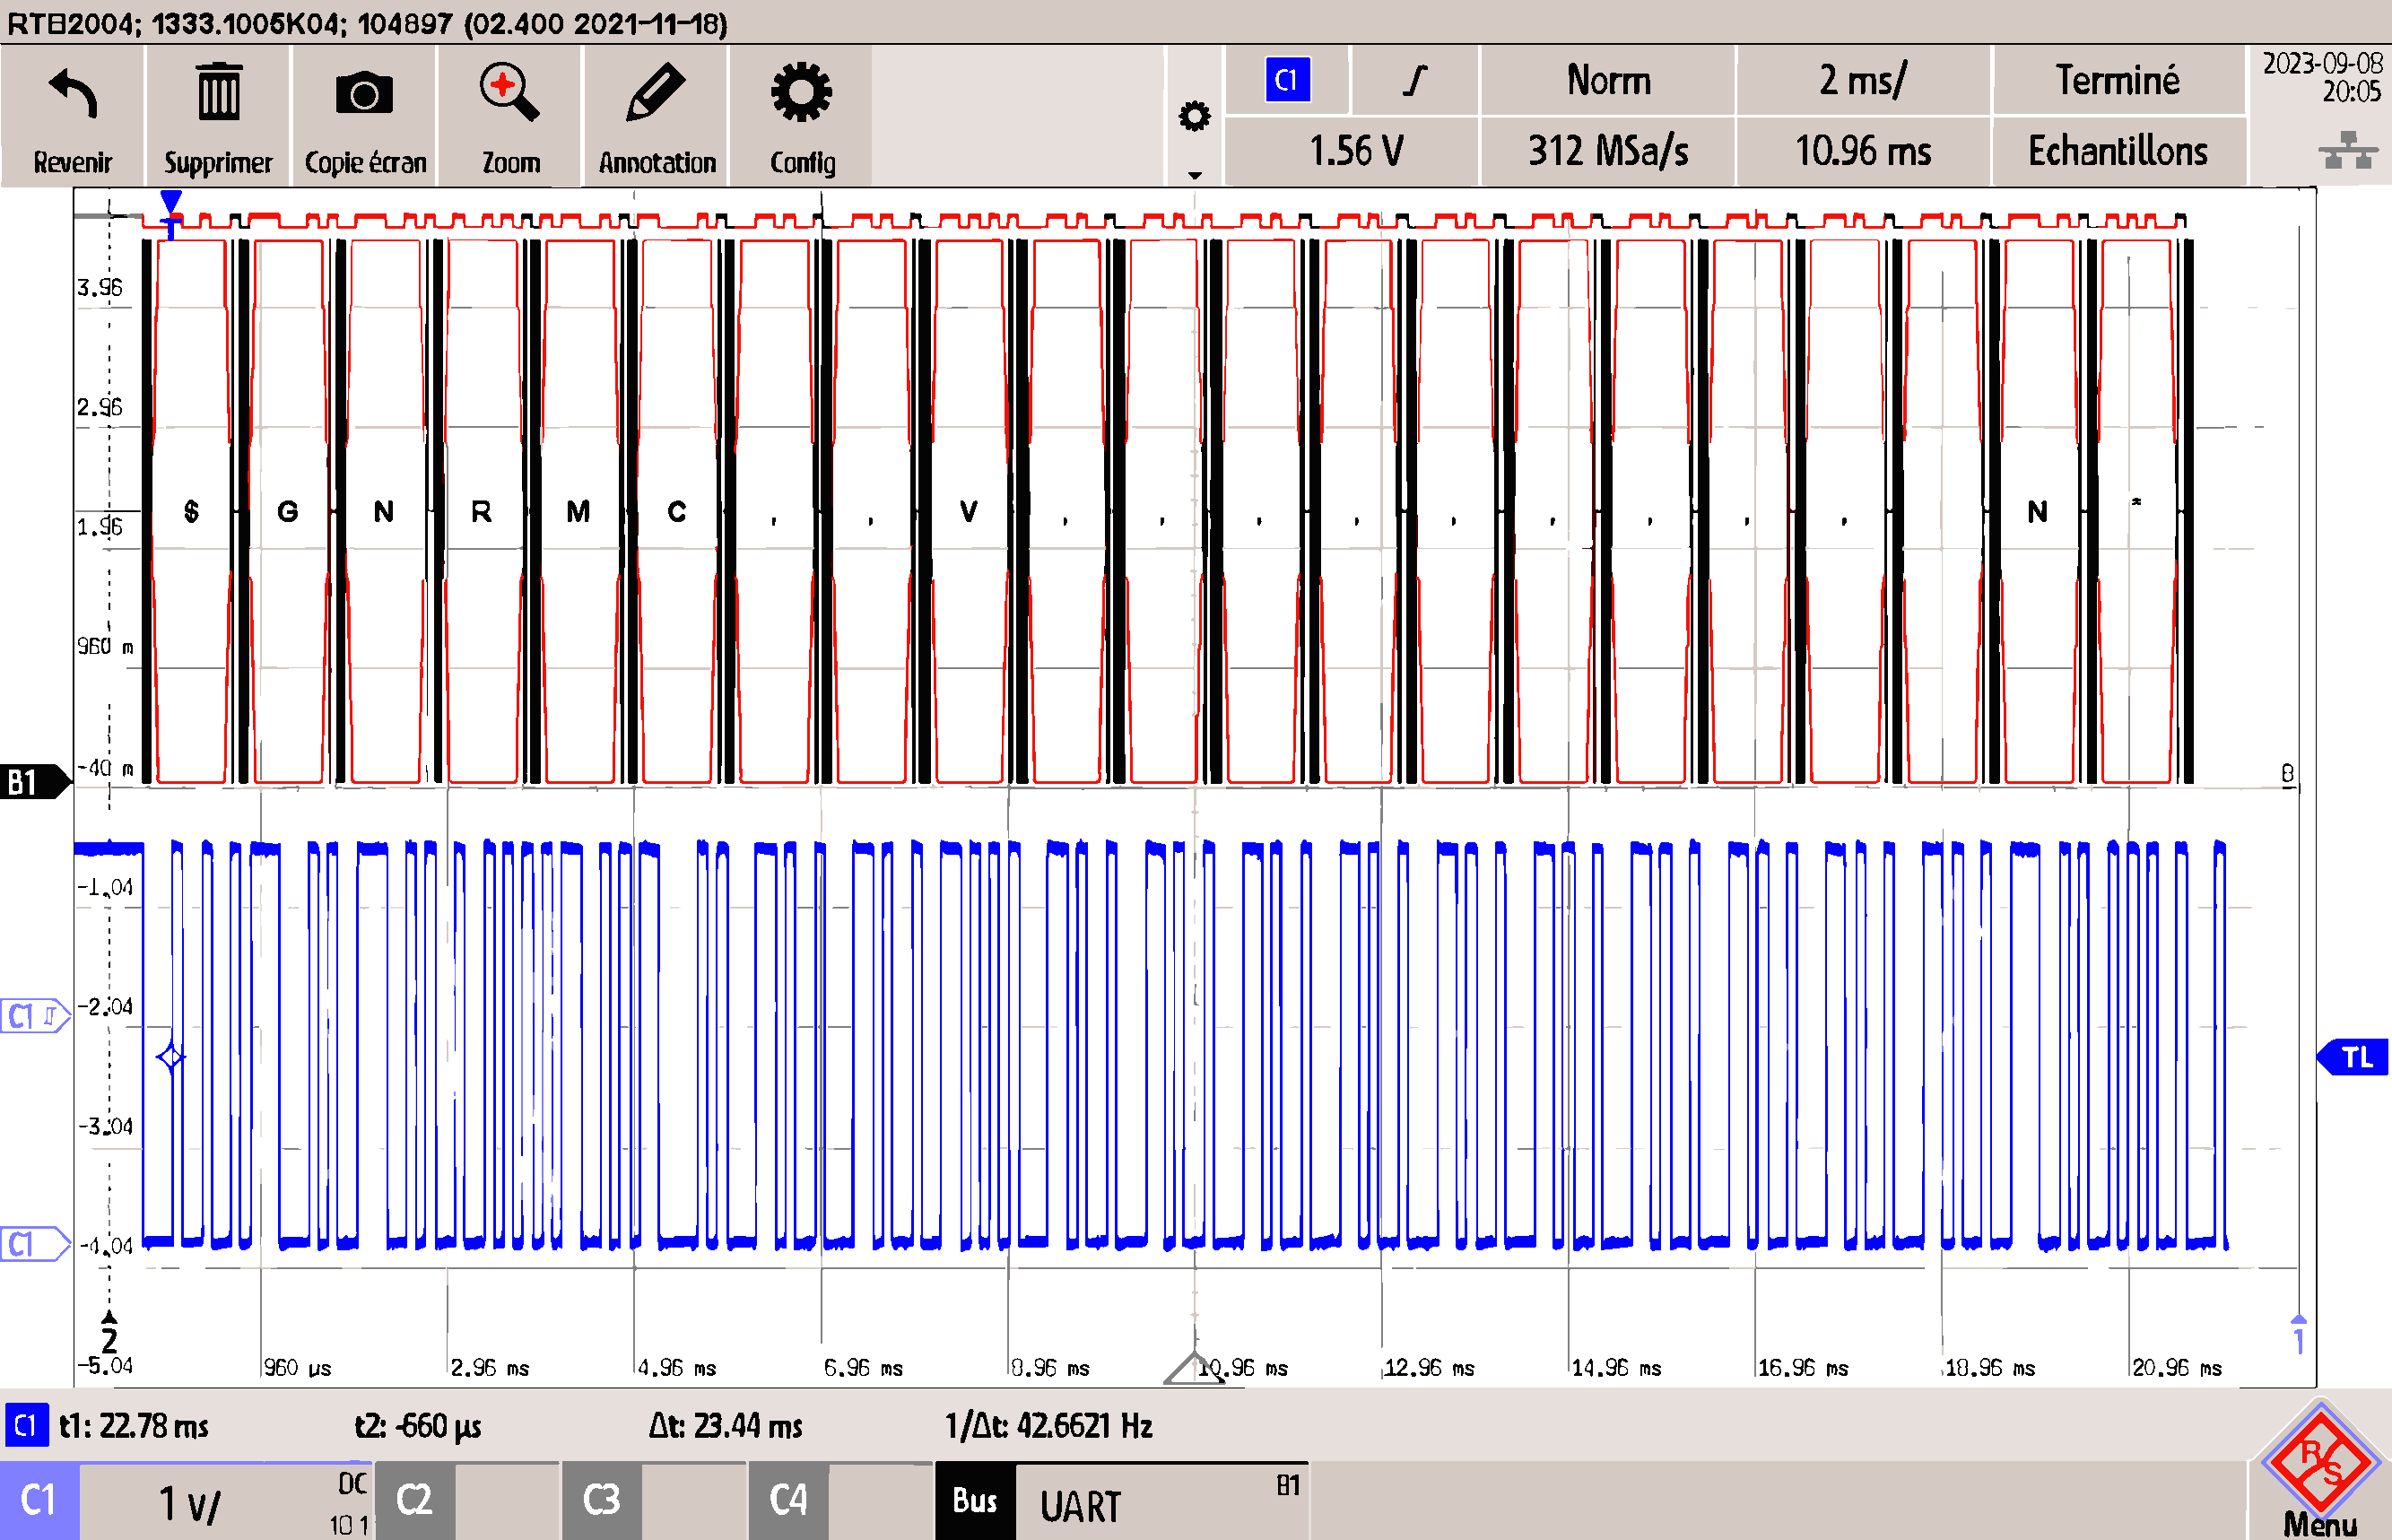
\includegraphics[width=0.7\linewidth]{../figures/mesures/UART/message-NMEA-RMC}
	\caption{Message RMC du protocole NMEA.}
	\label{fig:message-nmea-rmc}
	\source{Auteur}
\end{figure}

Nous observons sur la figure \ref{fig:message-nmea-rmc} le message décodé par l'oscilloscope \hyperref[ssec:Liste-materiel]{\textbf{P1}} : \textbf{\$GN\textcolor{blue}{RMC},,\textcolor{red}{V},,,,,,,,,N*}

\clearpage

\subsubsection{Communication UART2 FTDI} \label{ssec:Comm-UART2}
Dans cette section, nous examinerons les trames de communication sur l'UART 2, établies entre le \gls{mcu} et le \gls{FTDI}, qui sert de bus d'interface entre la boîte noire et un appareil externe.

\paragraph{Méthode de mesure} Ces mesures ont été effectuées pendant une communication entre la boîte noire et un ordinateur fixe, en utilisant l'application développée dans la section \ref{sec:devApp}.


\paragraph{Schéma de mesure} Le schéma de mesure est présenté sur figure \ref{fig:schema-mesure-ftdi} : 
\begin{figure}[h]
	\centering
	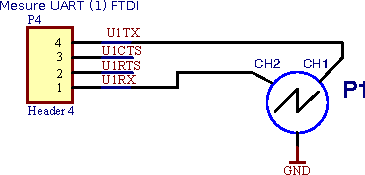
\includegraphics[width=.4\linewidth]{../figures/mesures/UART-FTDI/Schema-mesure-FTDI}
	\caption{Schéma de mesure UART2.}
	\label{fig:schema-mesure-ftdi}
	\source{Auteur}
\end{figure}

\paragraph{Mesures} Sur la figure \ref{fig:comm-uart2-config}, une communication est visible. Il s'agit d'une commande de configuration envoyée par l'application pour modifier le temps entre l'écriture des mesures \gls{gnss} à 5 secondes. Nous pouvons distinguer l'envoi de la commande "\textbf{INTG:5000}" et, \underline{$120\micro s$} après, la réception de la réponse de la boîte noire. Cela démontre une réactivité rapide du système dans le mode \textbf{CONFIG}.


\begin{figure}[h]
	\centering
	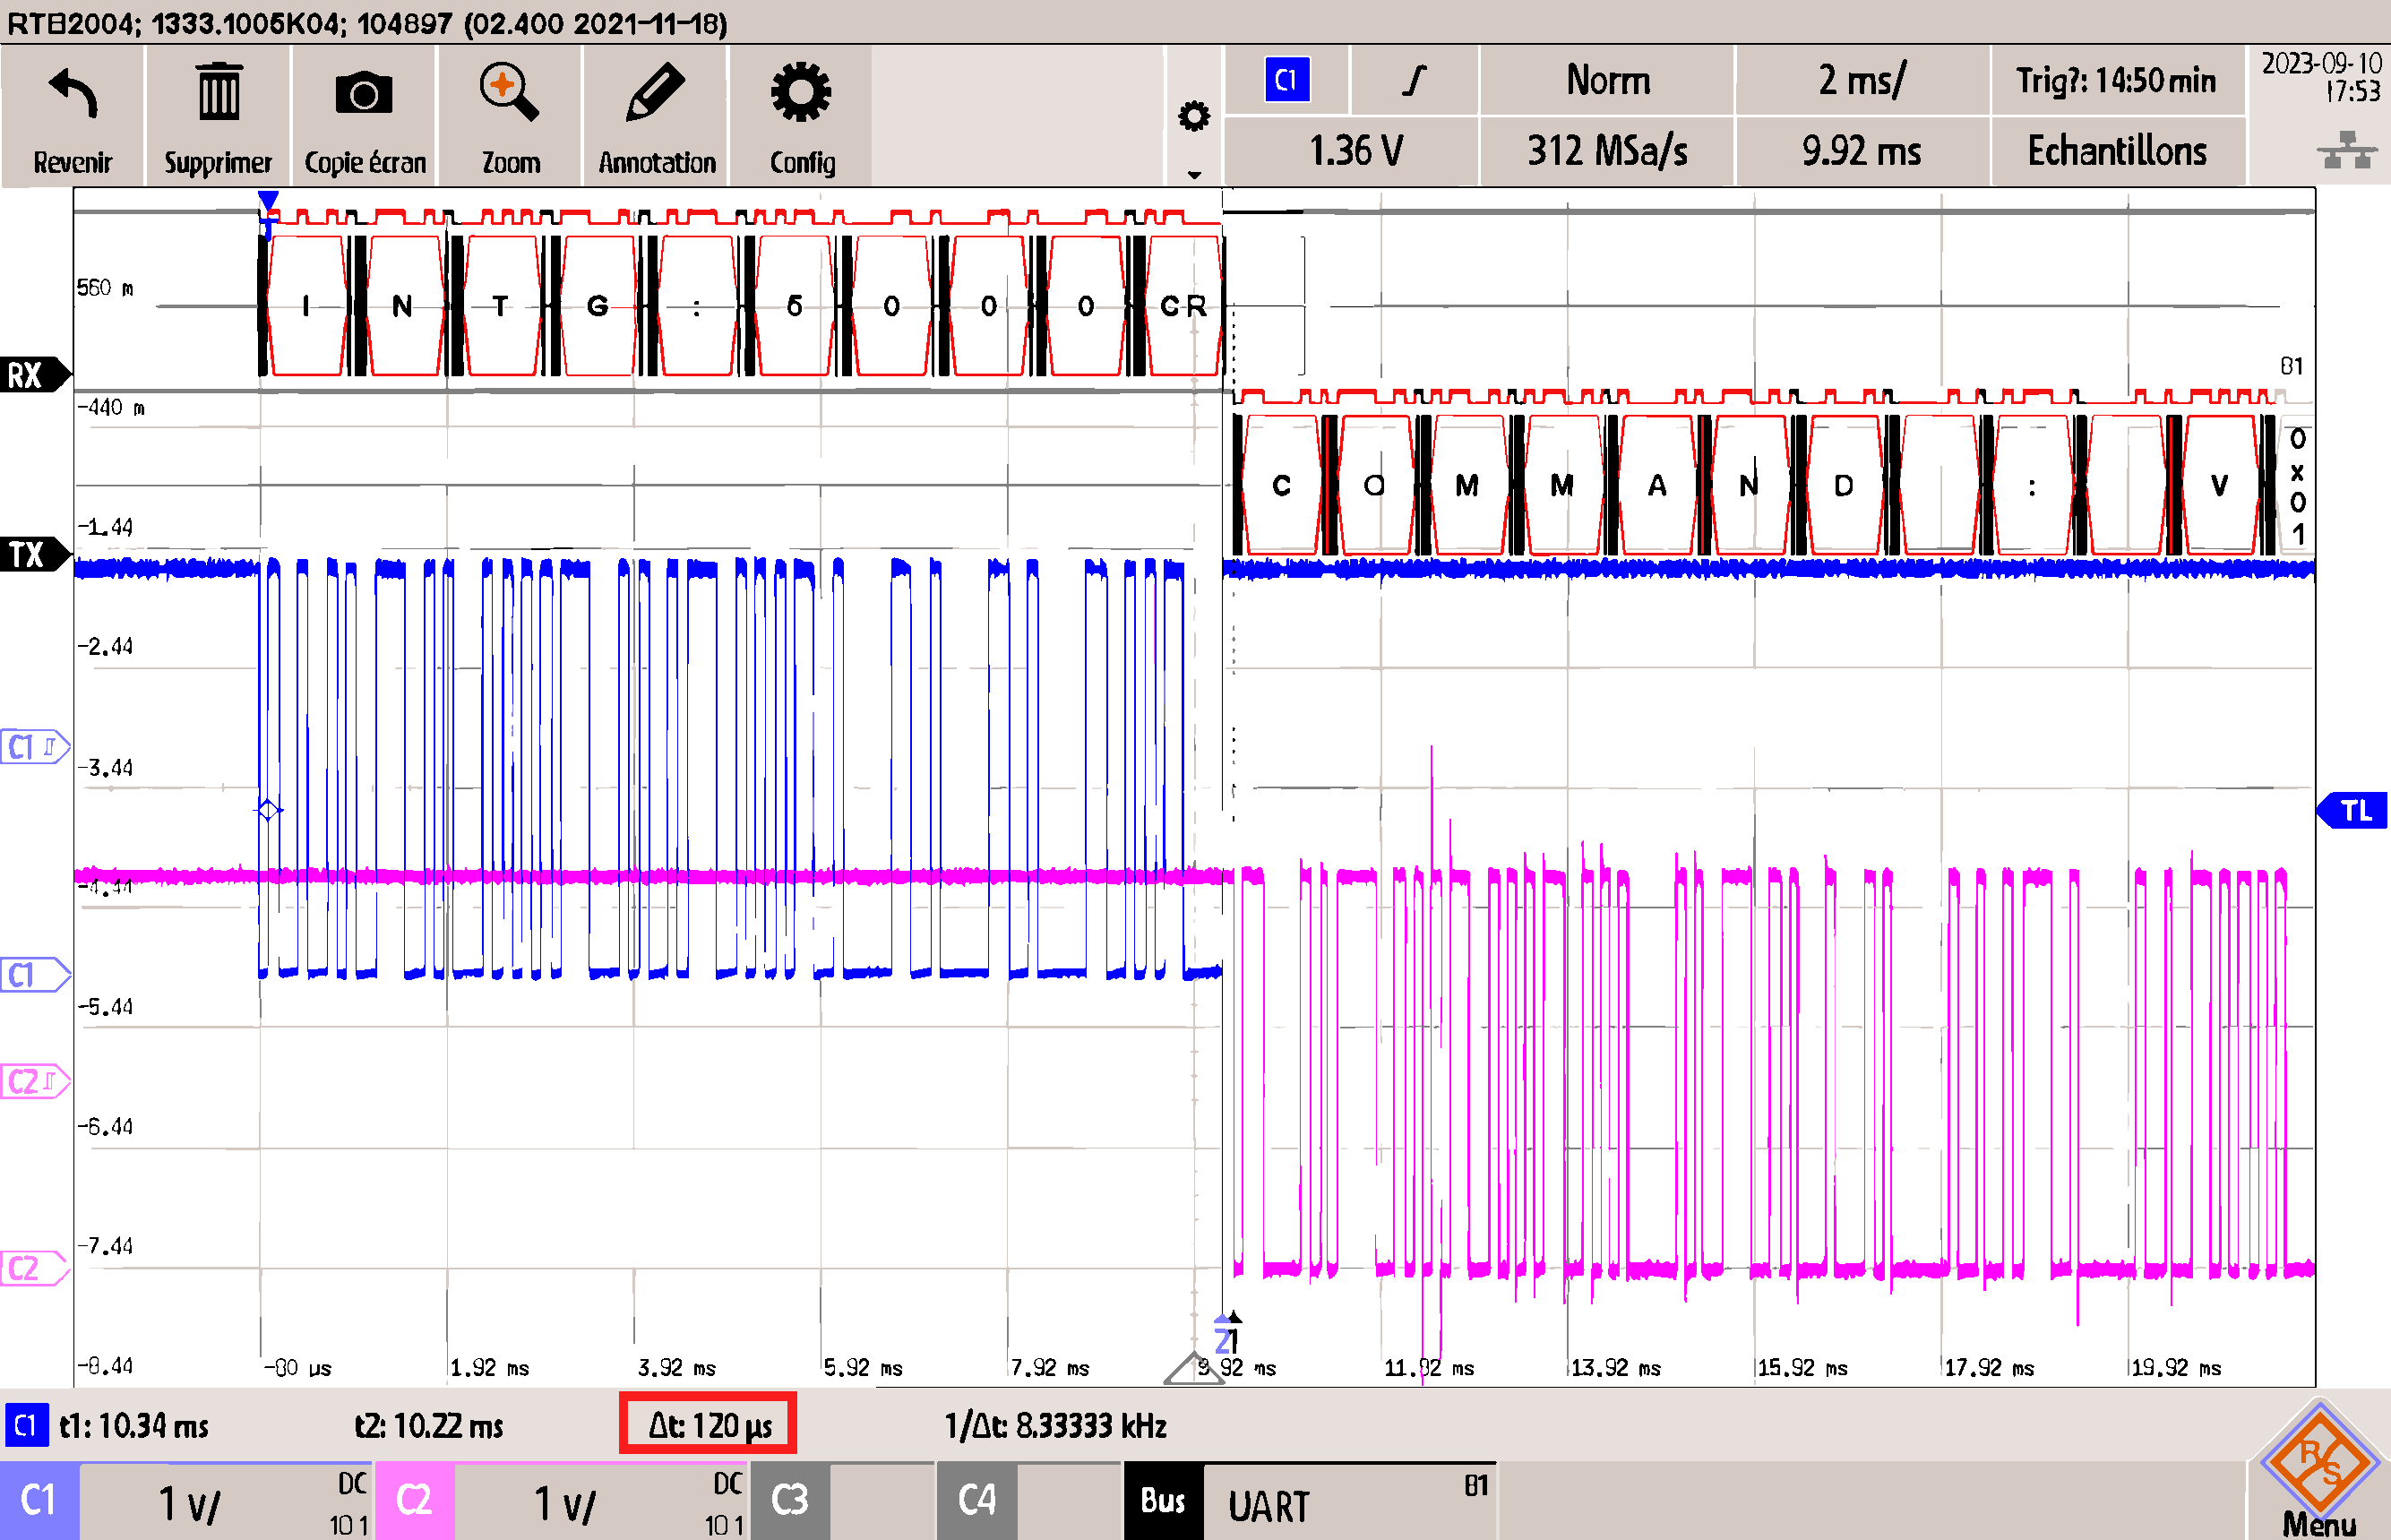
\includegraphics[width=0.7\linewidth]{../figures/mesures/UART-FTDI/comm-uart2-config}
	\caption{Trames configuration.}
	\label{fig:comm-uart2-config}
	\source{Auteur}
\end{figure}

\clearpage

Sur la figure \ref{fig:comm-uart-ecartlog}, nous observons le temps de réaction du système suite à une commande demandant l'obtention des LOGS de l'\gls{imu}. L'intervalle entre cette demande et la réponse du système en mode \textbf{LOGGING} est de \underline{$2.7ms$}, ce qui est plus élevé que la figure \ref{fig:comm-uart2-config}, sachant que le système à plus d'éléments à gérer lors de ce mode.


\begin{figure}[h]
	\centering
	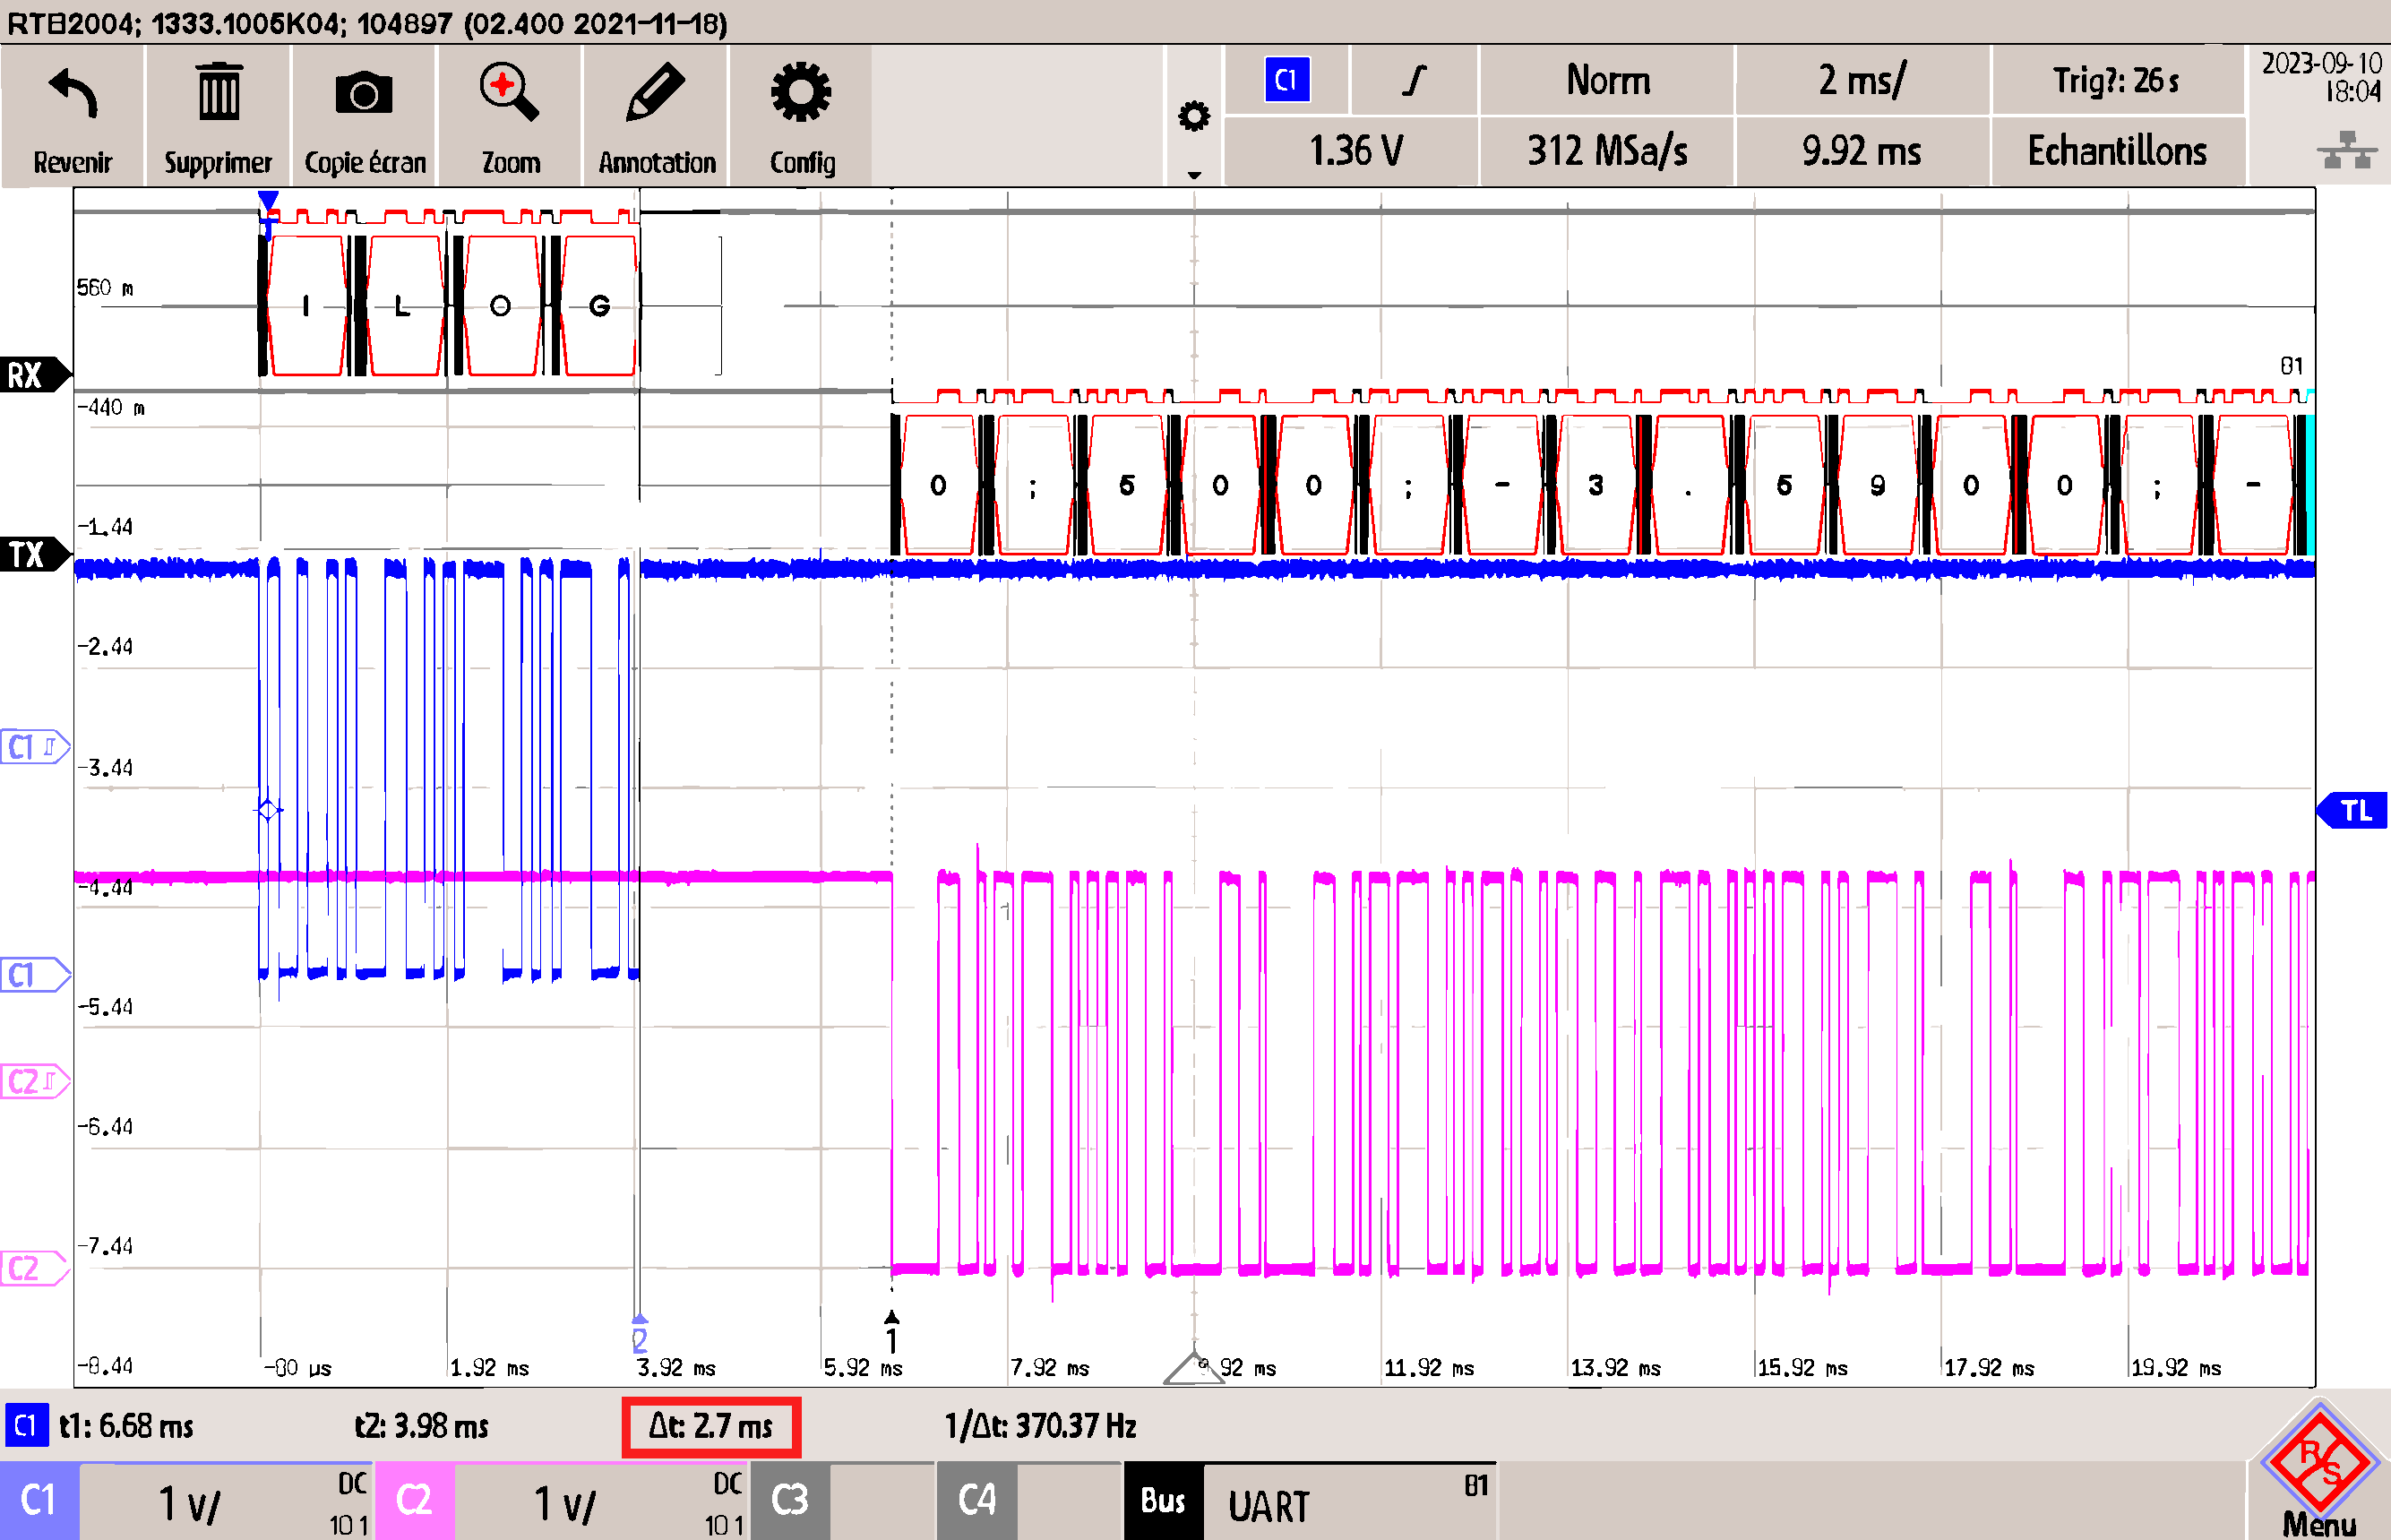
\includegraphics[width=0.7\linewidth]{../figures/mesures/UART-FTDI/comm-uart-ecartLog}
	\caption{Réaction commande durant \textbf{LOGGING}.}
	\label{fig:comm-uart-ecartlog}
	\source{Auteur}
\end{figure}



\subsubsection{Communication SPI, carte SD} \label{ssec:Comm-SPI}
Dans cette section, nous examinerons la communication SPI entre le \gls{mcu} et la carte SD.

\paragraph{Méthode de mesure} Étant donné la complexité de la communication SPI pour la gestion du système de fichiers FAT, notre objectif ici n'est pas d'analyser le protocole en lui-même, mais plutôt d'observer les signaux électriques lors du logging.

\paragraph{Schéma de mesure} Le schéma de mesure est visible sur la figure \ref{fig:schema-mesure-spi} :
\begin{figure}[h]
	\centering
	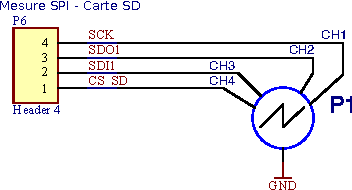
\includegraphics[width=0.5\linewidth]{../figures/mesures/SPI/Schema-mesure-spi}
	\caption{Schéma de mesure SPI.}
	\label{fig:schema-mesure-spi}
	\source{Auteur}
\end{figure}

\clearpage

\paragraph{Mesures} Sur la figure \ref{fig:densite-comm}, nous pouvons constater que la communication SPI est dense et constante durant le 

\begin{figure}[H]
	\centering
	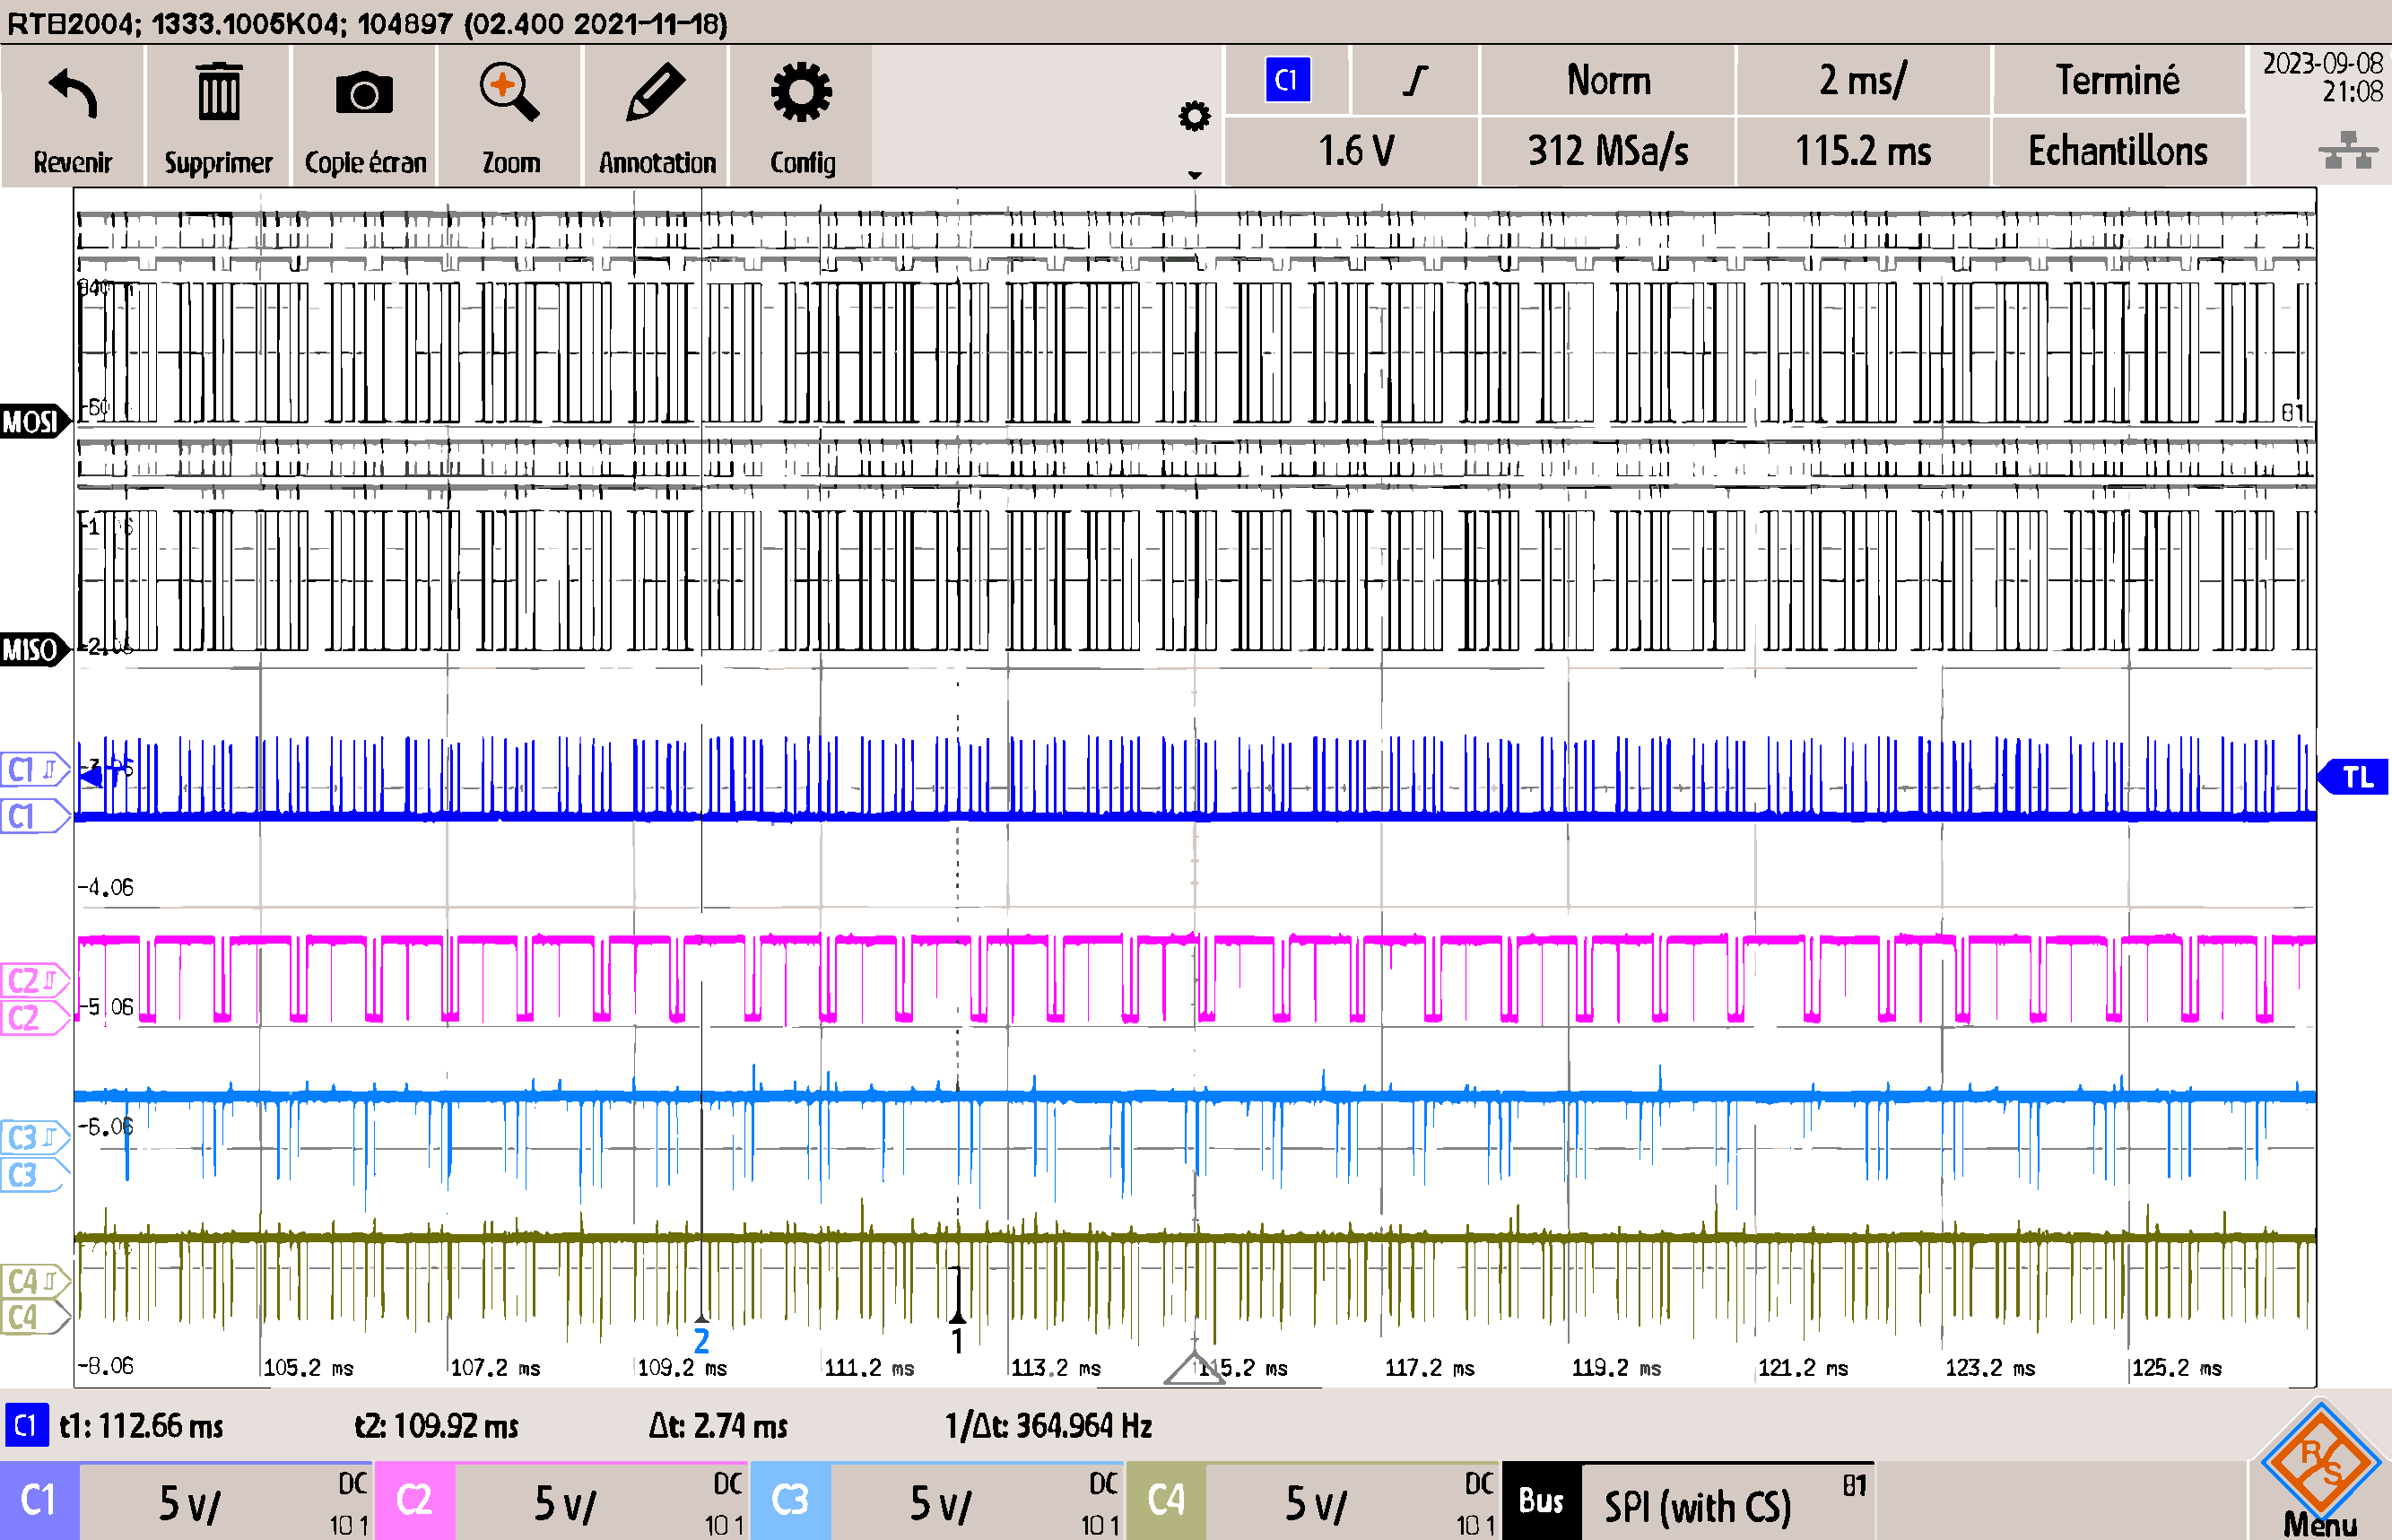
\includegraphics[width=0.7\linewidth]{../figures/mesures/SPI/densite-comm}
	\caption{Densité de la communication SPI.}
	\label{fig:densite-comm}
	\source{Auteur}
\end{figure}

\begin{figure}[H]
	\centering
	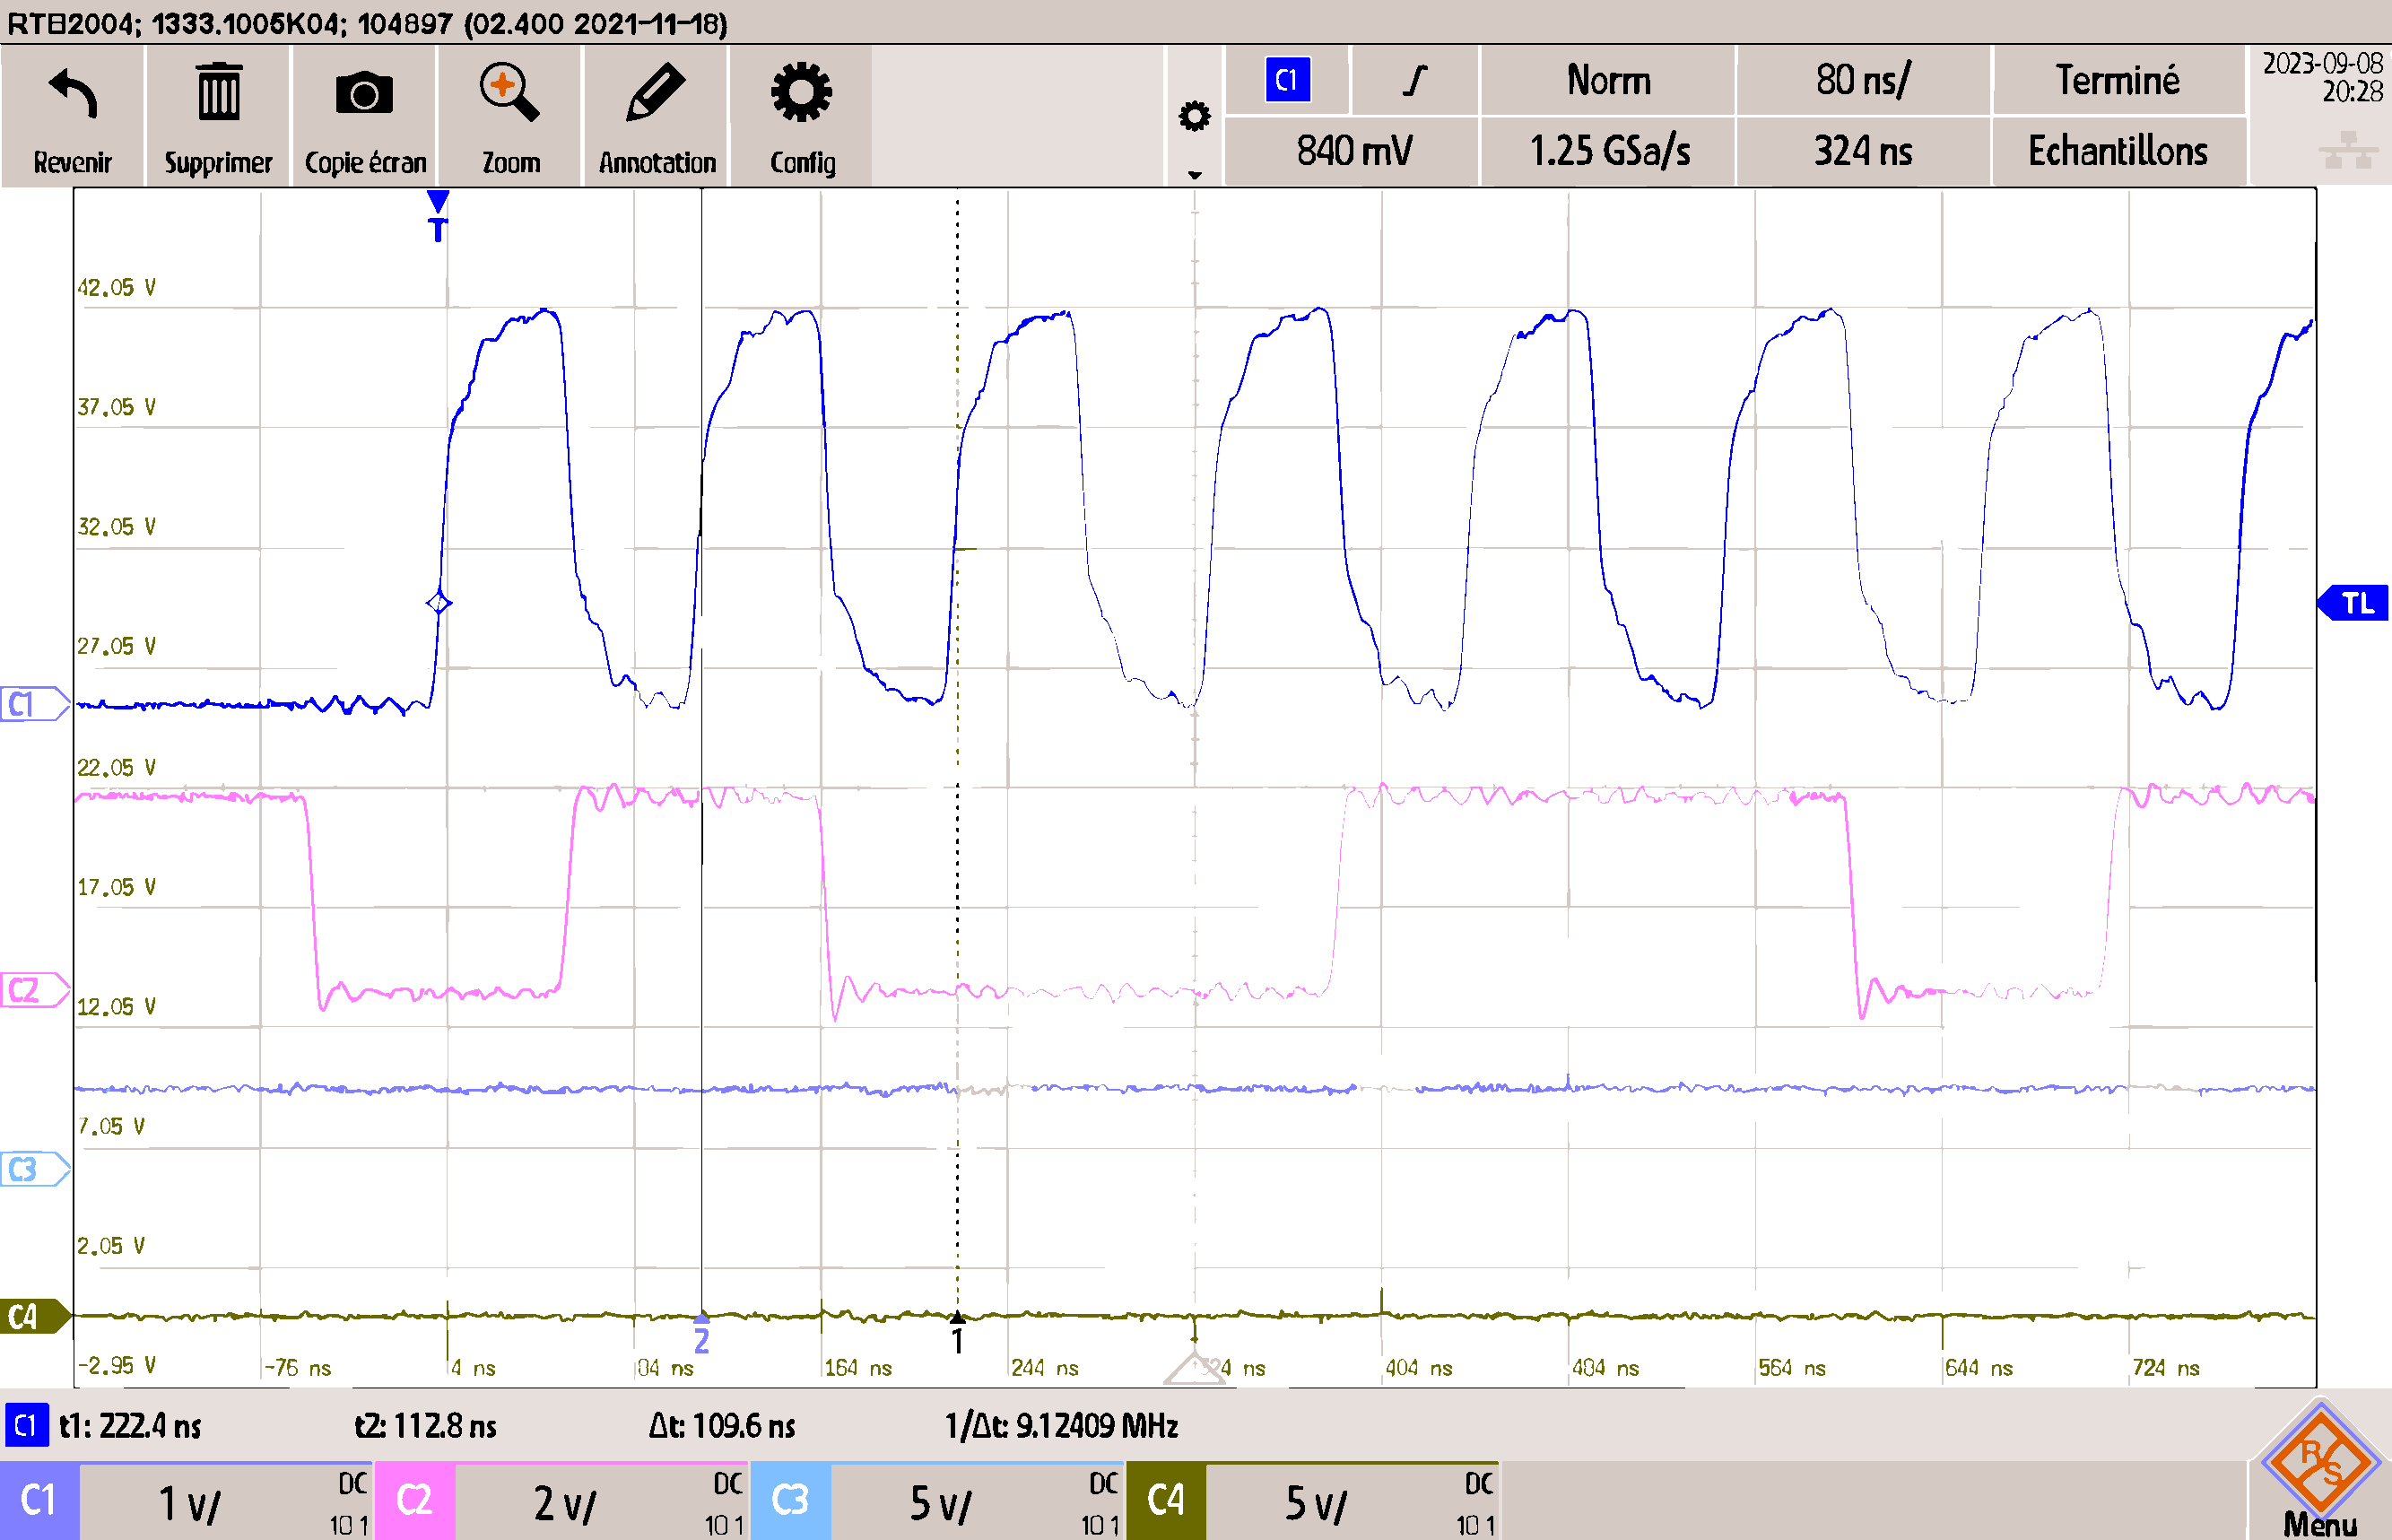
\includegraphics[width=0.7\linewidth]{../figures/mesures/SPI/freq-spi}
	\caption{Mesure fréquence clock SPI.}
	\label{fig:freq-spi}
	\source{Auteur}
\end{figure}





\section{Caractéristiques du produit fini} \label{sec:Carac-finis}